
\documentclass{beamer}

\usepackage{graphicx}
\usepackage{hyperref}
\usepackage[latin1]{inputenc}
\usepackage[T1]{fontenc}
\usepackage[english]{babel}
\usepackage{listings}
\usepackage{xcolor,mathrsfs,url}
\usepackage{amssymb}
\usepackage{amsmath}
\usepackage{ifthen}
\usepackage{subcaption}
%\usepackage{subfigure}
\usepackage{metricsbeamer} % using the metric beamer style
\usepackage{epstopdf} %use eps now!
%\usepackage{tikz}
%\usetikzlibrary{shapes.geometric, arrows}
\usepackage{blindtext}
\usepackage{pdflscape}
%\captionsetup{justification=centering}

\usepackage{lvblisting}


% Avoid dancing decimals
\usepackage{siunitx}
% Make plusminus signs work in table/tabular
\sisetup{separate-uncertainty=true}

%%%%%%%%%%%%%%%%%%%%%%%%%%%%%%%%%

\newcommand{\highlight}[1]{%
  \colorbox{red!50}{$\displaystyle#1$}}
\newcommand{\midbarnew}{}
\newcommand{\subsec}[1]%


%%%%%%%%%%%%%%%%%%%%%%%%%%%%%%%%%

\definecolor{blue2}{RGB}{0,102,204}
\definecolor{green}{RGB}{0,204,102}
\definecolor{red}{RGB}{204,0,0}
\definecolor{mygray1}{gray}{0.4}
\definecolor{mygray2}{gray}{0.2}
%%%%%%%%%%%%%%%%%%%%%%%%%%%%%%%%%


\pgfdeclareimage[height=0.5cm]{logosmall}{Fig/logosmall}
\pgfdeclareimage[height=4cm]{logobig}{Fig/logos}

% use this number to modify the scaling of the headline on titlepage
\def\titlescale{1}

\def\authora{\color{blue} Daniel Traian Pele, 
	\color{black}Niels Wesselh�fft, Wolfgang K. H�rdle,\color{brown} Yannis Yatracos, \color{purple} Michalis Kolossiatis}

\def\authorb{\footnotesize{\color{black}International Research Training Group 1792\\
Ladislaus von Bortkiewicz Chair of Statistics \\
Humboldt--Universit�t zu Berlin \\
\medskip


 \color{blue}Department of Statistics and Econometrics \\
Bucharest University of Economic Studies\\
\medskip
\color{purple}Department of Mathematics and Statistics\\ University of Cyprus, Nicosia\\
\medskip
\color{brown} Yau Mathematical Sciences Center, Tsinghua University, Beijing, China}}


%\def\linka{http://lvb.wiwi.hu-berlin.de}
%\def\linkb{http://www.case.hu-berlin.de}
%\def\linkc{http://irtg1792.hu-berlin.de}
%\def\email{}	% Your email address

%%%%%%%%%%%%%%%%%%%%%%%%%%%%%%%%%

\title[]{Are Cryptos becoming alternative Assets?}


\begin{document}
\Section{}

\frame[plain]{% create the titleslide, layout controlled in metricsbeamer
	\titlepage
}

%%%%%%%%%%%%%%%%%%%%%%%%%%%%%%%%%

\section{Motivation}\label{sec:motivation}

\frame{
\frametitle{Genus differentia approach}

\begin{figure}[!ht]
\centering
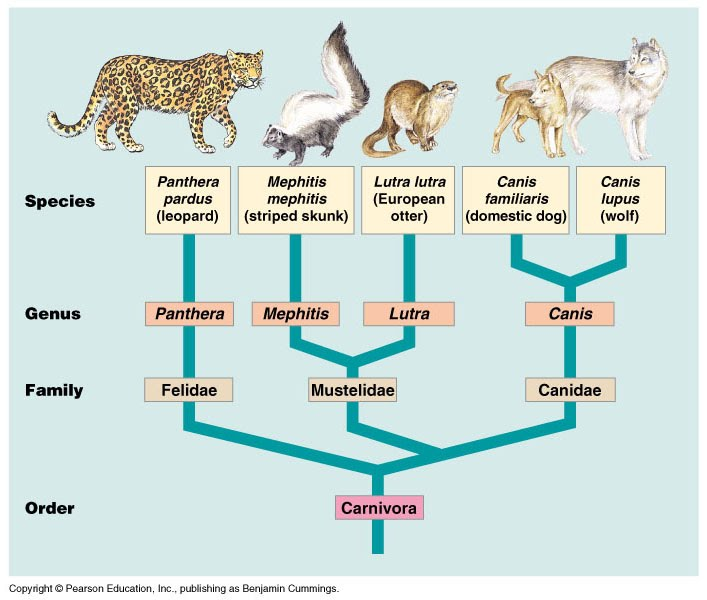
\includegraphics[width=0.6\textwidth]{Fig/intro_bio} %
\caption{Genus differentia approach in biology}
%\hyperlink{sec:appendix_stable}{\beamergotobutton{Stable laws}}}
\end{figure}
}

\frame{
\frametitle{Genus differentia approach}

\begin{figure}[!ht]
\centering
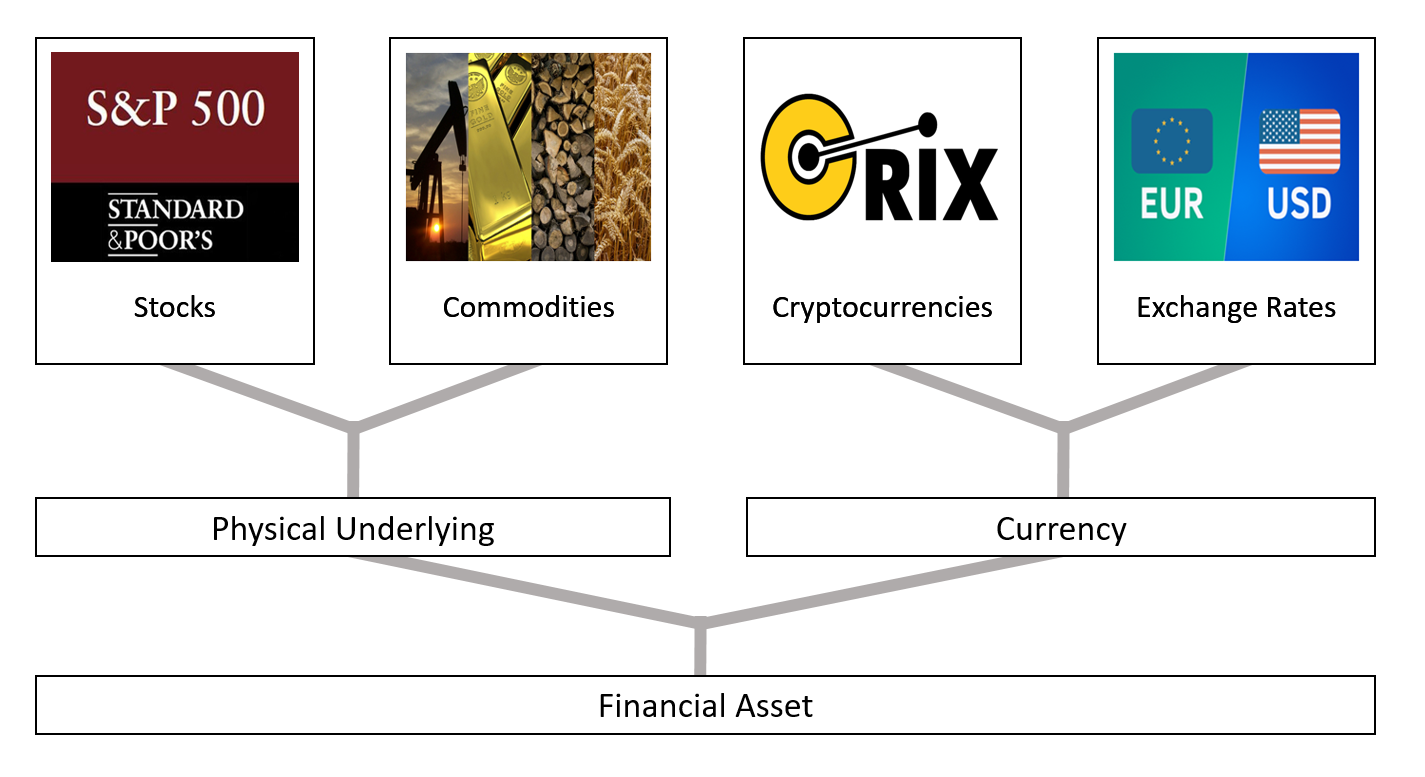
\includegraphics[width=1\textwidth]{Fig/intro_fin} %
\caption{Genus differentia approach in finance}
%\hyperlink{sec:appendix_stable}{\beamergotobutton{Stable laws}}}
\end{figure}
}

%%%%%%%%%%%%%%%%%%%%%%%%%%%%%%%%

\frame{
\frametitle{Aim of classification}

\begin{itemize}
  \item Genotypic differentiation
\begin{itemize}
  \item Biology - the change in DNA sequences.
  \item Finance - the underlying process of price manifestation.
\end{itemize}
\item Phenotypic differentiation
\begin{itemize}
  \item Biology - classification based on behavior and features of a species.
  \item Finance - classification based on statistical features of the price series.
\end{itemize}

\end{itemize}

}

\frame{
	\frametitle{Motivation}
	\begin{itemize}\small{
	\item Question: What defines cryptocurrencies?}
\end{itemize}
\begin{figure}[!aristotel]


\includegraphics[width=0.30\textwidth]{Fig/mining}
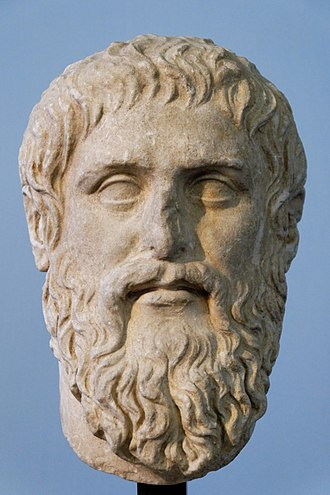
\includegraphics[width=0.08\textwidth]{Fig/plato}
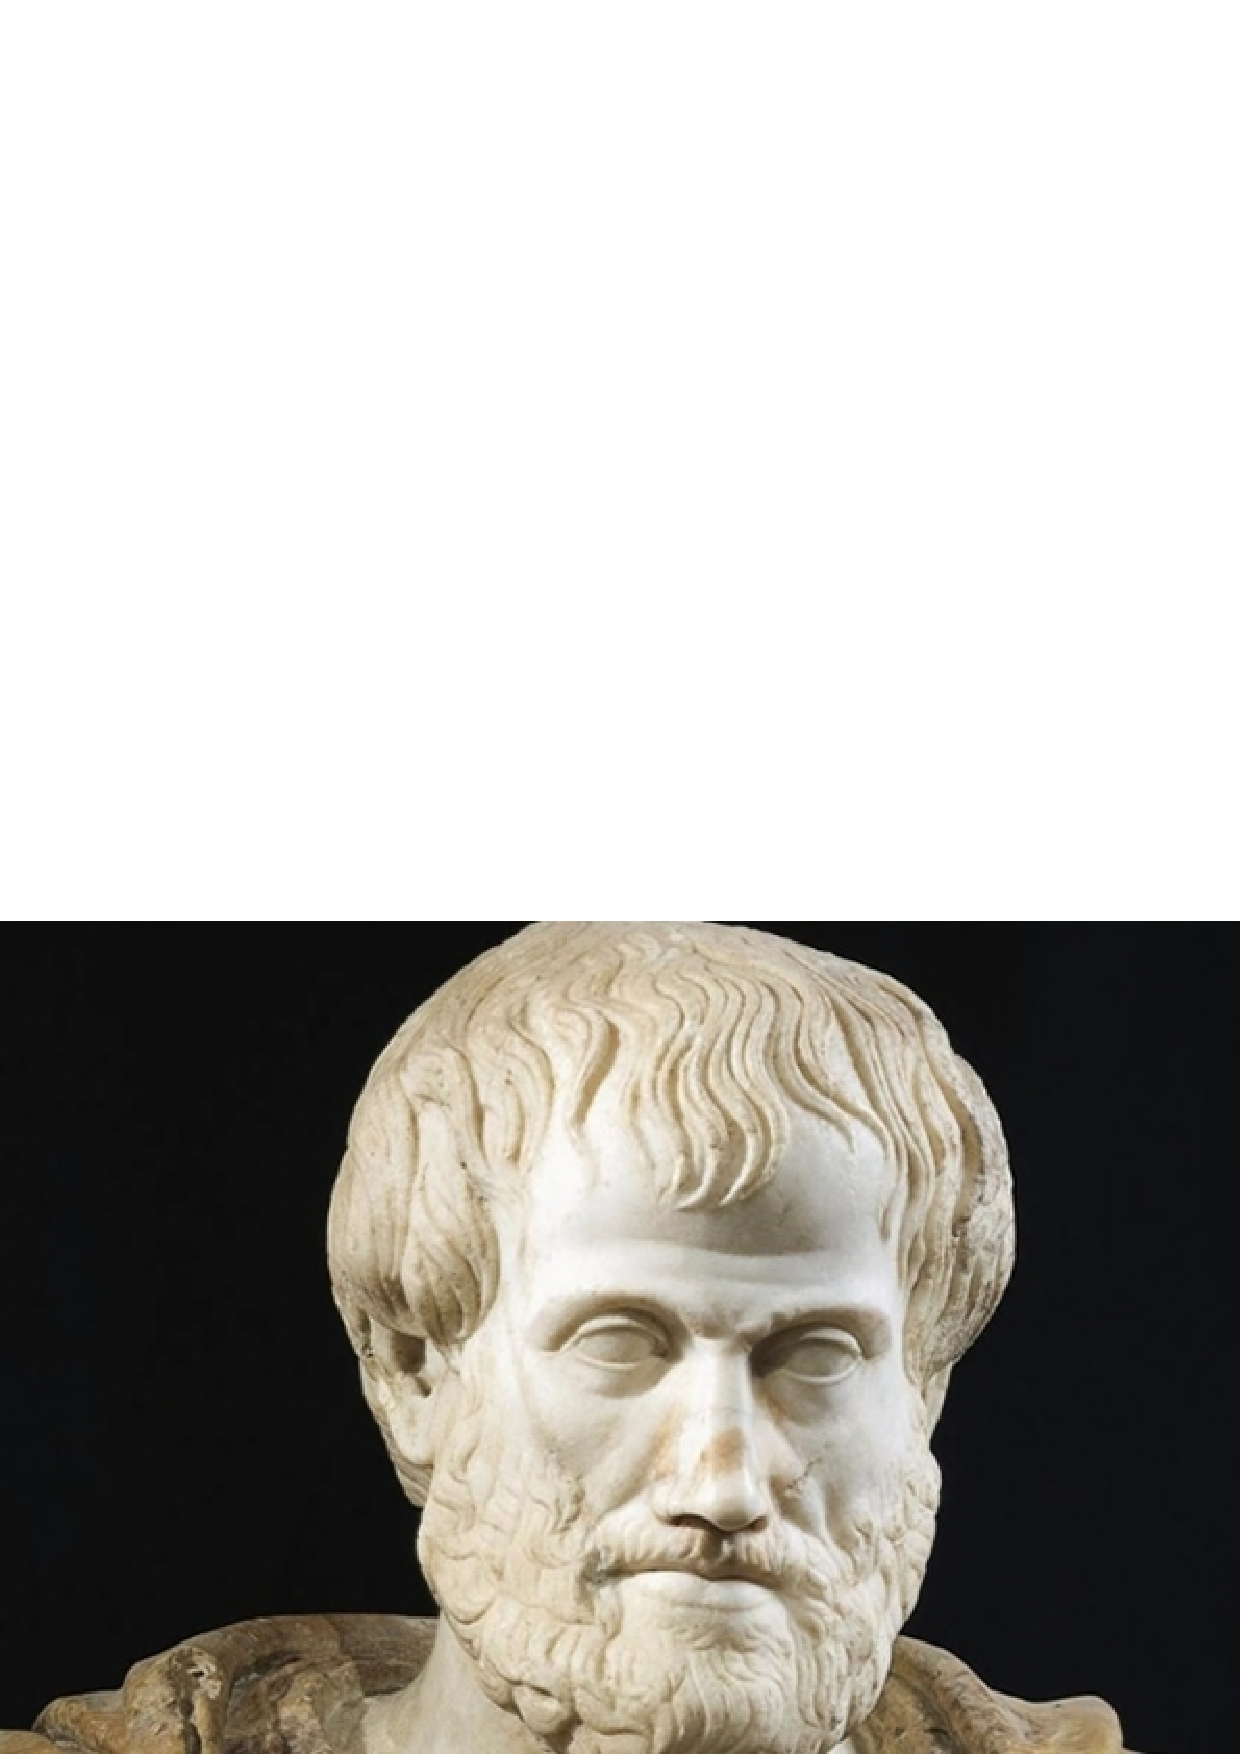
\includegraphics[width=0.200\textwidth]{Fig/aristotel}
\end{figure}

	\begin{itemize}\small{
		\item Plato: man is an upright, featherless biped, with broad, fat nails.
		\item Aristotle: definition of a species consists of genus proximum and differentia specifica.

			\item Goal: Define cryptocurrencies in terms of their genus proximum and differentia specifica.

			\item Method: Find latent variables, to form groups of shared characteristics.

		\item Finding: Synchronic evolution, i.e. asymptotic speciation.

	\item Implication: Cryptocurrencies are a different species in the ecosystem of financial instruments.}
\end{itemize}
}

%%%%%%%%%%%%%%%%%%%%%%%%%%%%%%%%%

\frame{
\thispagestyle{empty}
\frametitle{Outline}
\begin{enumerate}
  \item Motivation
  \item Data and descriptives
  \item Factor model
  \item Explanation
  \item Expanding window
  \item Conclusion
\end{enumerate}
}
%%%%%%%%%%%%%%%%%%%%%%%%%%%%%%%%



%%%%%%%%%%%%%%%%%%%%%%%%%%%%%%%%


\frame{
	\frametitle{Literature review}

	\begin{itemize}
		\item Dyhrberg (2016): BTC has similarities to both GOLD and the USD, being in between a currency and a commodity.
	\end{itemize}
	\begin{itemize}
		\item Baur et al. (2018): BTC volatility and correlation characteristics are distinctively different compared to GOLD and USD.
	\end{itemize}
	\begin{itemize}
		\item H�rdle et al. (2018): BTC, XRP, LTC, ETH returns exhibit higher volatility, skewness and kurtosis compared to GOLD and S\&P500 daily returns.
	\end{itemize}
	\begin{itemize}
		\item Henriques et al. (2018): BTC can serve as a substitute for GOLD in a portfolio.
	\end{itemize}
		\begin{itemize}
		\item Zhang et al. (2018): Cryptocurrencies presents heavier tails and higher Hurst exponent than the classical assets.
	\end{itemize}


}

%%%%%%%%%%%%%%%%%%%%%%%%%%%%%%%%
\section{Data and descriptives}\label{sec:data}

\frame{
\frametitle{Data}
\begin{itemize}
	\item Sample: $n=679$ \href{https://github.com/QuantLet/Genus_proximum_cryptos/blob/master/list.xlsx}
	{\color{blue}{assets.}}
\end{itemize}

\begin{itemize}
	
\item New asset class
\begin{itemize}
\item Cryptocurrencies: $n_1=150$ 
\end{itemize}
\end{itemize}
\begin{itemize}
\item Old asset classes
\begin{itemize}
\item Stocks (S\&P 500): $n_2=496$
\item Exchange rates: $n_3=13$ \hyperlink{sec:appendix_forex}{\beamergotobutton{List}}
\item Commodities (Bloomberg Commodity Index): $n_4=20$ \hyperlink{sec:appendix_Commodities}{\beamergotobutton{List}}
\end{itemize}
\end{itemize}
\begin{itemize}
\item Daily data from 01/02/2014 - 08/30/2019 (1426 trading days).
%\begin{itemize}
%	\item 5 trading days/week for stocks, exchange rates and commodities
%	\item 7 trading days/week for cryptocurrencies
\end{itemize}

}






%%%%%%%%%%%%%%%%%%%%%%%%%%%%%%%%

\frame{
\frametitle{Statistical assessment}

\begin{itemize}
  \item Return $X$ is a r.v. with cdf $F()$ from which $p=23$ statistics are estimated.
  \item Moments of order $k\in\mathbb{R}^+$, $\mu_k=\mathop{\mbox{\sf E}}\left\{(X-\mu\right)^k\}$.
\begin{itemize}
\item variance: $\sigma^{2}=E\left\{{(X-\mu)}^2\right\}$ ;
\item skewness:  $Skewness=E\left\{{(X-\mu)}^3\right\}/{\sigma}^{3}$;
\item kurtosis: $Kurtosis =E\left\{{(X-\mu)}^4\right\}/{\sigma}^{4}$.
\end{itemize}
\item Tails: $\alpha \in\{0.005,0.01,0.025,0.05,0.95,0.975,0.99,0.995\}$.
\begin{itemize}
  \item $Q_\alpha=\inf\left\{x\in\mathbb{R}:\alpha\leq F(x)\right\}$;
  \item $CTE_\alpha=\begin{cases}
    \mathop{\mbox{\sf E}}\left\{X\mid X<Q_\alpha\right\}, & \alpha<0.5\\
    \mathop{\mbox{\sf E}}\left\{X\mid X>Q_\alpha\right\}, & \alpha>0.5
  \end{cases}$
\end{itemize}
\item Scaling and memory parameters
\begin{itemize}
\item Alpha-stability \hyperlink{sec:appendix_stable}{\beamergotobutton{Alpha-stability}}
\item ARCH parameter (GARCH (1,1))
\item GARCH parameter (GARCH (1,1))
\end{itemize}
\end{itemize}
}


\frame{
\frametitle{Assets profile}
\begin{table}[!ht]
	\centering
	\label{table:table_4}
	\scriptsize{\tiny{
		\begin{tabular}{l S[table-format=3.2, round-mode=places,round-precision=3] S[table-format=3.2, round-mode=places,round-precision=3] S[table-format=3.2, round-mode=places,round-precision=3] S[table-format=3.2, round-mode=places,round-precision=3]
				S[table-format=3.2, round-mode=places,round-precision=2]}\hline\hline
			\multicolumn{1}{l}{\bfseries Variable} &\multicolumn{1}{l}{\bfseries Commodities}&\multicolumn{1}{l}{\bfseries Cryptocurrencies} &\multicolumn{1}{l}{\bfseries Exchange rates} &\multicolumn{1}{l}{\bfseries Stocks} \\ \hline
			$\sigma^2\cdot10^{3}$                  & 0.365 & 14.563 & 0.028 & 0.27\\
			$Skewness$ & 0.245 & 0.723 & -1.233 & -0.52\\
			$Kurtosis$ & 22.461 & 28.037 & 38.201 & 13.392\\
			$Stable_\alpha$                & 1.721 & 1.41 & 1.714 & 1.711\\
			$Stable_\gamma$           & 0.01 & 0.047 & 0.003 & 0.009\\
			$Q_{5\%}$                & -0.027 & -0.159 & -0.008 & -0.025\\
			$Q_{2.5\%}$                & -0.034 & -0.21 & -0.01 & -0.033\\
			$Q_{1\%}$                & -0.044 & -0.296 & -0.013 & -0.044\\
			$Q_{0.5\%}$                & -0.054 & -0.378 & -0.015 & -0.054\\
			$CTE_{5\%}$                & -0.038 & -0.25 & -0.011 & -0.038\\
			$CTE_{2.5\%}$                & -0.047 & -0.319 & -0.014 & -0.047\\
			$CTE_{1\%}$                & -0.06 & -0.428 & -0.017 & -0.062\\
			$CTE_{0.5\%}$                & -0.073 & -0.525 & -0.021 & -0.076\\
			$Q_{95\%}$                & 0.026 & 0.169 & 0.008 & 0.024\\
			$Q_{97.5\%}$                & 0.034 & 0.243 & 0.01 & 0.03\\
			$Q_{99\%}$                & 0.046 & 0.364 & 0.013 & 0.04\\
			$Q_{99.5\%}$                & 0.057 & 0.48 & 0.015 & 0.049\\
			$CTE_{95\%}$                & 0.039 & 0.297 & 0.011 & 0.034\\
			$CTE_{97.5\%}$                & 0.049 & 0.393 & 0.013 & 0.042\\
			$CTE_{99\%}$                & 0.064 & 0.544 & 0.016 & 0.055\\
			$CTE_{99.5\%}$                & 0.08 & 0.671 & 0.018 & 0.066\\
			GARCH parameter & 0.706 & 0.796 & 0.728 & 0.637\\
			ARCH parameter & 0.118 & 0.159 & 0.078 & 0.13\\ \hline \hline
	\end{tabular}}}
\caption{ Assets profile}
\end{table}
}




%%%%%%%%%%%%%%%%%%%%%%%%%%%%%%%%

\section{Classification}\label{sec:classification}

\frame{
\frametitle{Factor analysis}



\begin{itemize}
  \item Estimate the correlation matrix for all variables.
  \item Factor extraction based on the correlation of the coefficients.
  \item Factor rotation.

\end{itemize}

}


\frame{
\frametitle{Correlation matrix}

\begin{figure}[!ht]
\centering
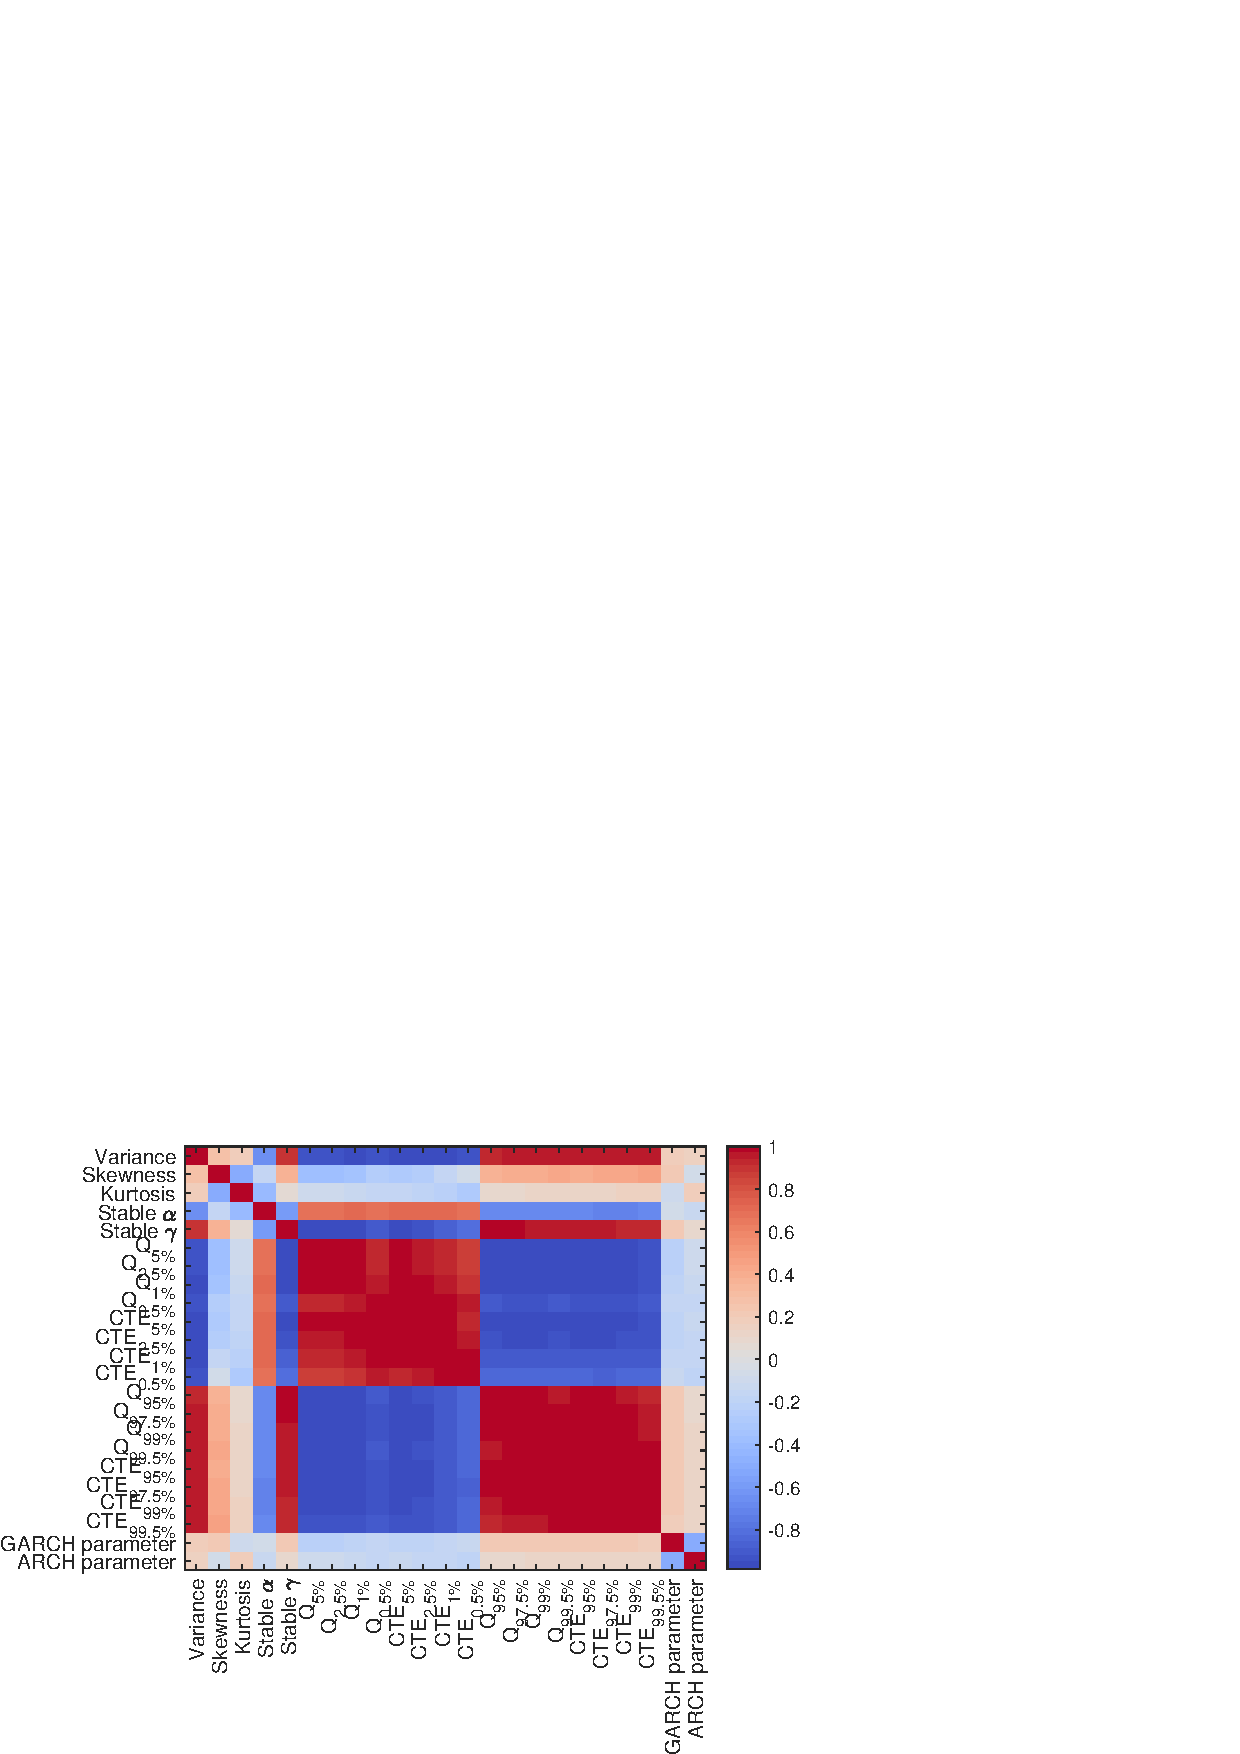
\includegraphics[width=0.7\textwidth]{Fig/figure_1}
\caption{\centering Correlation matrix of the statistical estimates. \href{https://github.com/QuantLet/Genus_proximum_cryptos/tree/master/SFA_Cryptos}{
\includegraphics[width=0.03\textwidth]{Fig/qloqo}\ SFA\_cryptos}
}
\end{figure}

}

%%%%%%%%%%%%%%%%%%%%%%%%%%%%%%%%



\frame{
\frametitle{Factor model}

\begin{itemize}
  \item Linear Factor model


\begin{align}
X=QF+\mu+\varepsilon,\ \varepsilon\sim{G()}
\end{align}

\begin{itemize}
  \item $X$ is the initial matrix of $p$ variables
  \item $Q$ is a matrix of the non-random loadings
  \item $F$ are the common $k$ factors ($k<p$)
  \item	$\mu$ is the vector of the means of initial $p$ variables
  \item $\varepsilon$ is a matrix of the random specific factors
  \item Random vectors $F$ and $U$ are unobservable and uncorrelated
\end{itemize}
\end{itemize}

}

\frame{
\frametitle{Factor model extensions}

\begin{itemize}
\item Time-varying factor model
\begin{align}
X_t=Q_tF_t+\mu_t+\varepsilon_t,\ \varepsilon_t\sim{G()}
\end{align}
\item Nonlinearities in the factors
\begin{align}
X=Q m(F)+\mu+\varepsilon,\ \varepsilon\sim{G()}
\end{align}
\item General nonlinear
\begin{align}
X=m(F)+\varepsilon,\ \varepsilon\sim{G()},
\end{align} where $m()$ is a function
\end{itemize}

}
%%%%%%%%%%%%%%%%%%%%%%%%%%%%%%%%

\frame{
\frametitle{Factors loadings and scree plot}
\begin{figure}[!ht]
	\begin{minipage}[b]{0.48\textwidth}
		\centering
		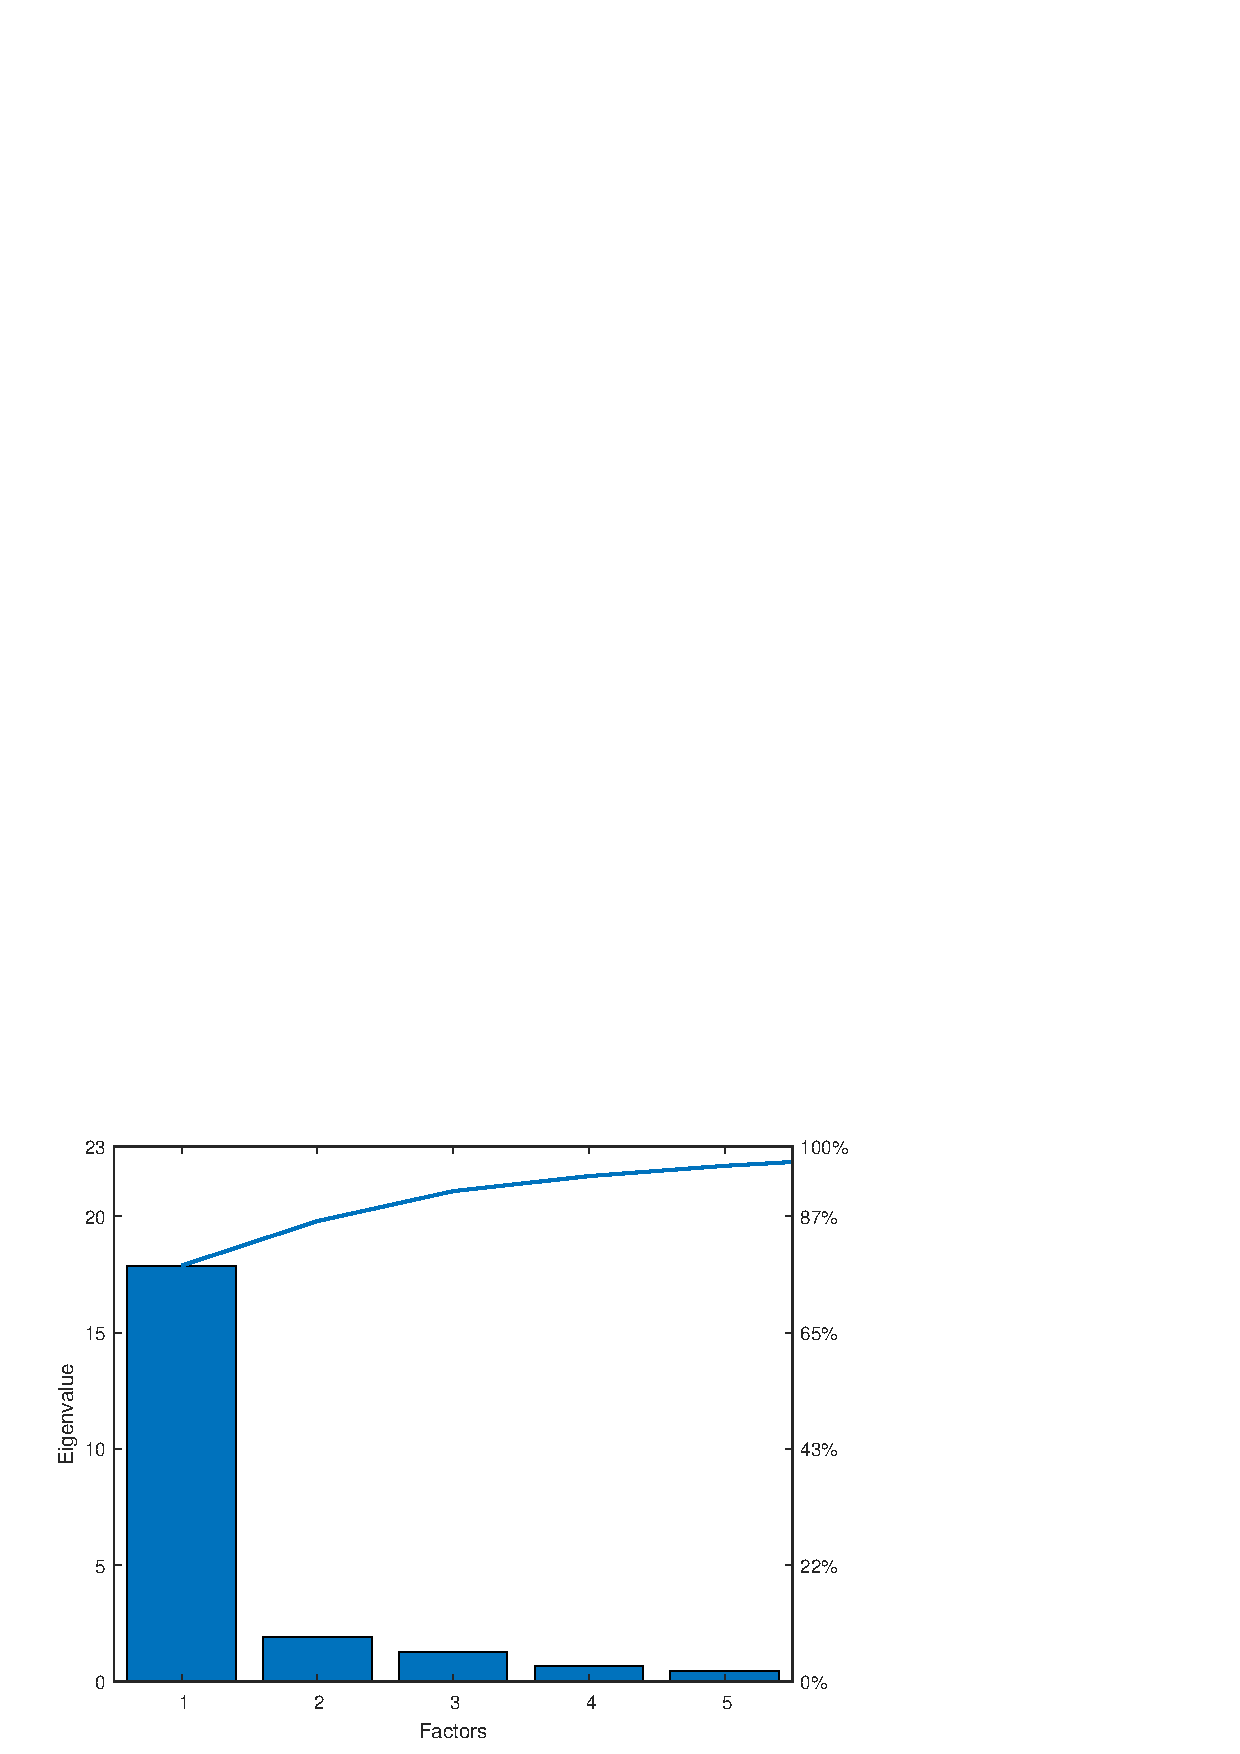
\includegraphics[width=1\textwidth]{Fig/figure_2}
		
		\label{fig:1}
	\end{minipage}
	\begin{minipage}[b]{0.48\textwidth}
		\centering
		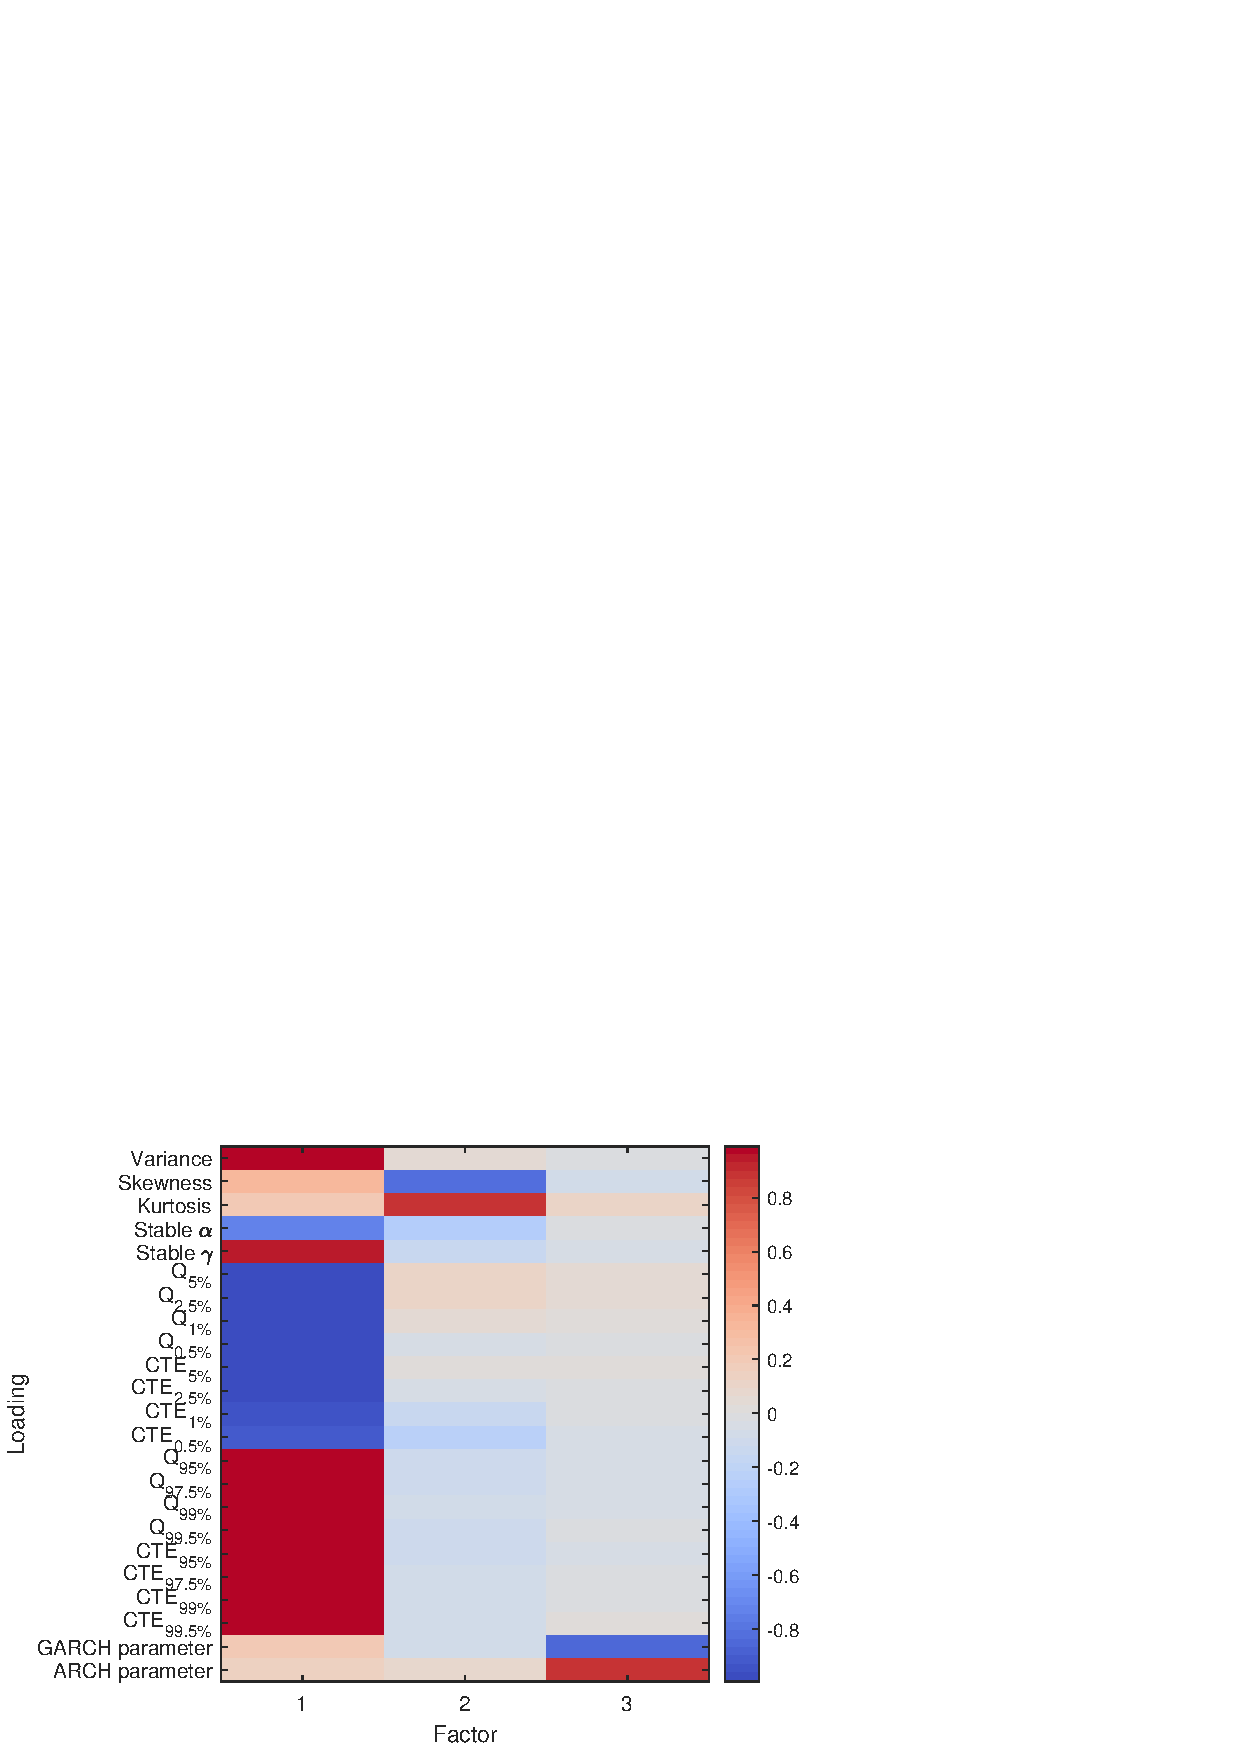
\includegraphics[width=1\textwidth]{Fig/figure_3}
	\end{minipage}
\caption{Scree plot and factors loadings. \href{https://github.com/QuantLet/Genus_proximum_cryptos/tree/master/SFA_Cryptos}{
\includegraphics[width=0.03\textwidth]{Fig/qloqo}\ SFA\_cryptos}
}
\end{figure}


}


\frame{
	\frametitle{Mapping of the factors}
	
	\begin{enumerate}
		\item Tail factor - 77\% of the total variance
		
			\begin{itemize}
				\item Alpha-stable parameters $S_\alpha$, $S_\gamma$
			\end{itemize}
			\begin{itemize}
				\item Lower and upper quantiles
			\end{itemize}
			\begin{itemize}
				\item Conditional tail expectations
			\end{itemize}
					\begin{itemize}
			\item Variance
		\end{itemize}


	\item Moment factor - 8\% of the total variance

	\begin{itemize}
		\item Skewness
	\end{itemize}
	\begin{itemize}
	\item Kurtosis
\end{itemize}

\item Memory factor - 6\% of the total variance




\begin{itemize}
	\item ARCH parameter
\end{itemize}

\begin{itemize}
	\item GARCH parameter
\end{itemize}
\end{enumerate}
}
%%%%%%%%%%%%%%%%%%%%%%%%%%%%%%%%

\frame{
\frametitle{Tail factor vs Moment factor}

\begin{figure}[!ht]
	\begin{minipage}[b]{0.48\textwidth}
	\centering
	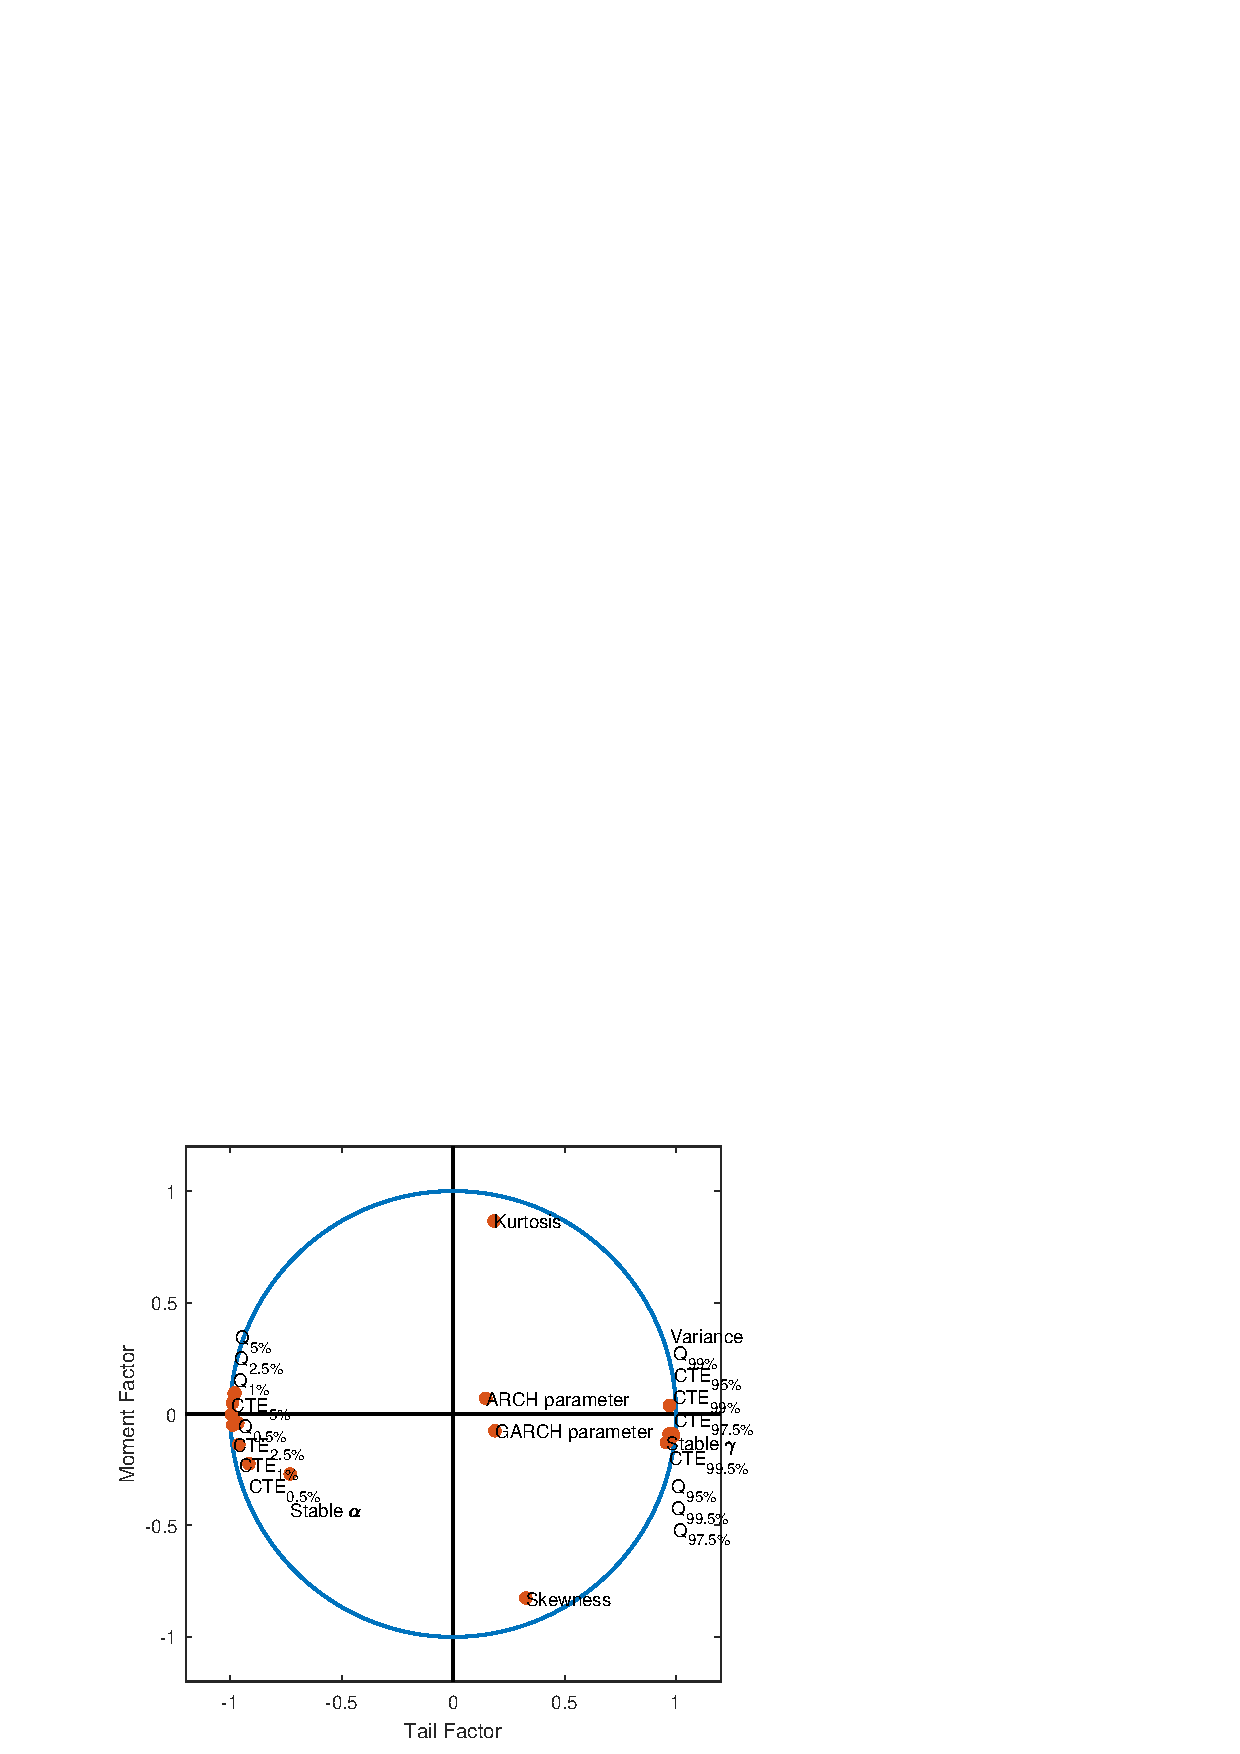
\includegraphics[width=1\textwidth]{Fig/figure_4a}
	
	
\end{minipage}
\begin{minipage}[b]{0.48\textwidth}
	\centering
	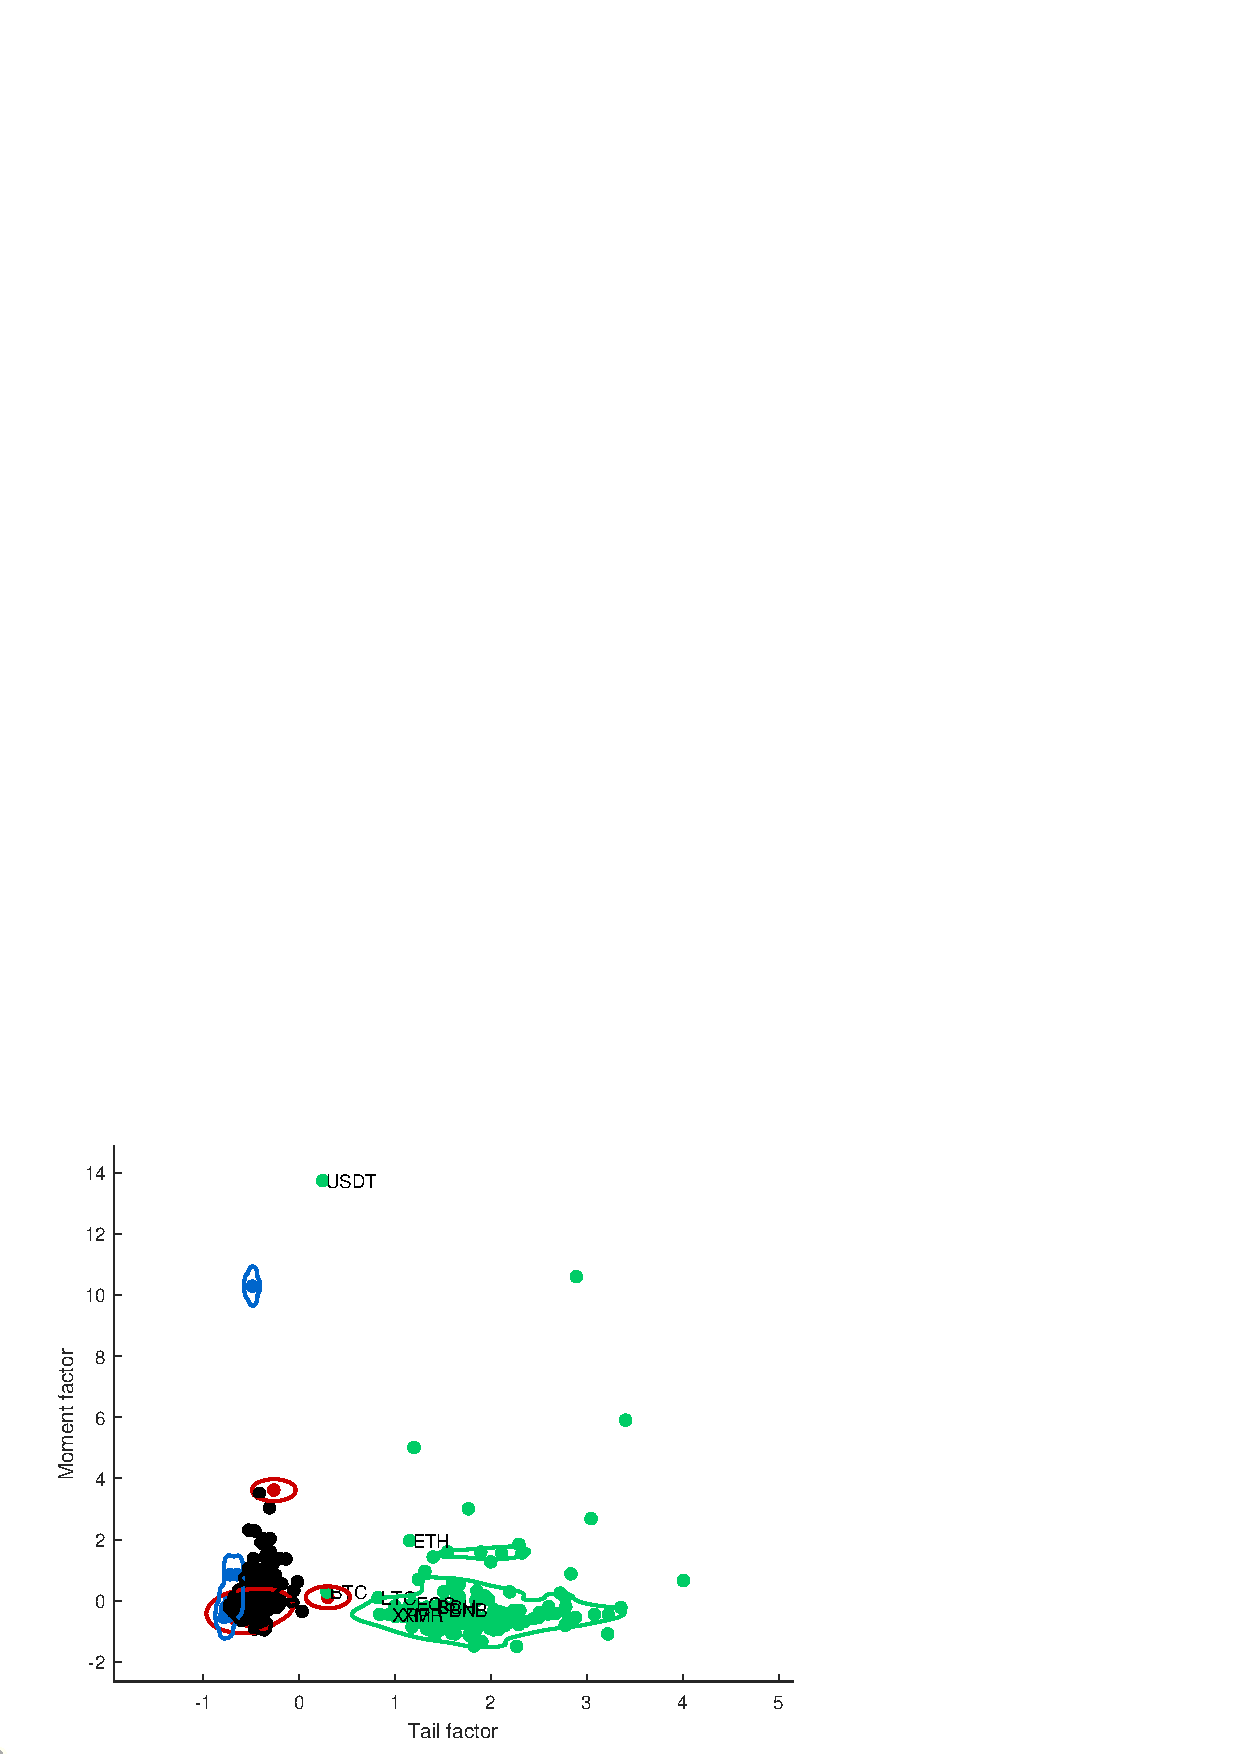
\includegraphics[width=1\textwidth]{Fig/figure_4b}
	
\end{minipage}
\caption {Loadings (left) and scores (right) based on tail and moment factor. \href{https://github.com/QuantLet/Genus_proximum_cryptos/tree/master/SFA_cryptos}{
\includegraphics[width=0.03\textwidth]{Fig/qloqo}\ SFA\_cryptos}}
\end{figure}

}

%%%%%%%%%%%%%%%%%%%%%%%%%%%%%%%%

\frame{
\frametitle{Tail factor vs Memory factor}

\begin{figure}[!ht]
	\begin{minipage}[b]{0.48\textwidth}
	\centering
	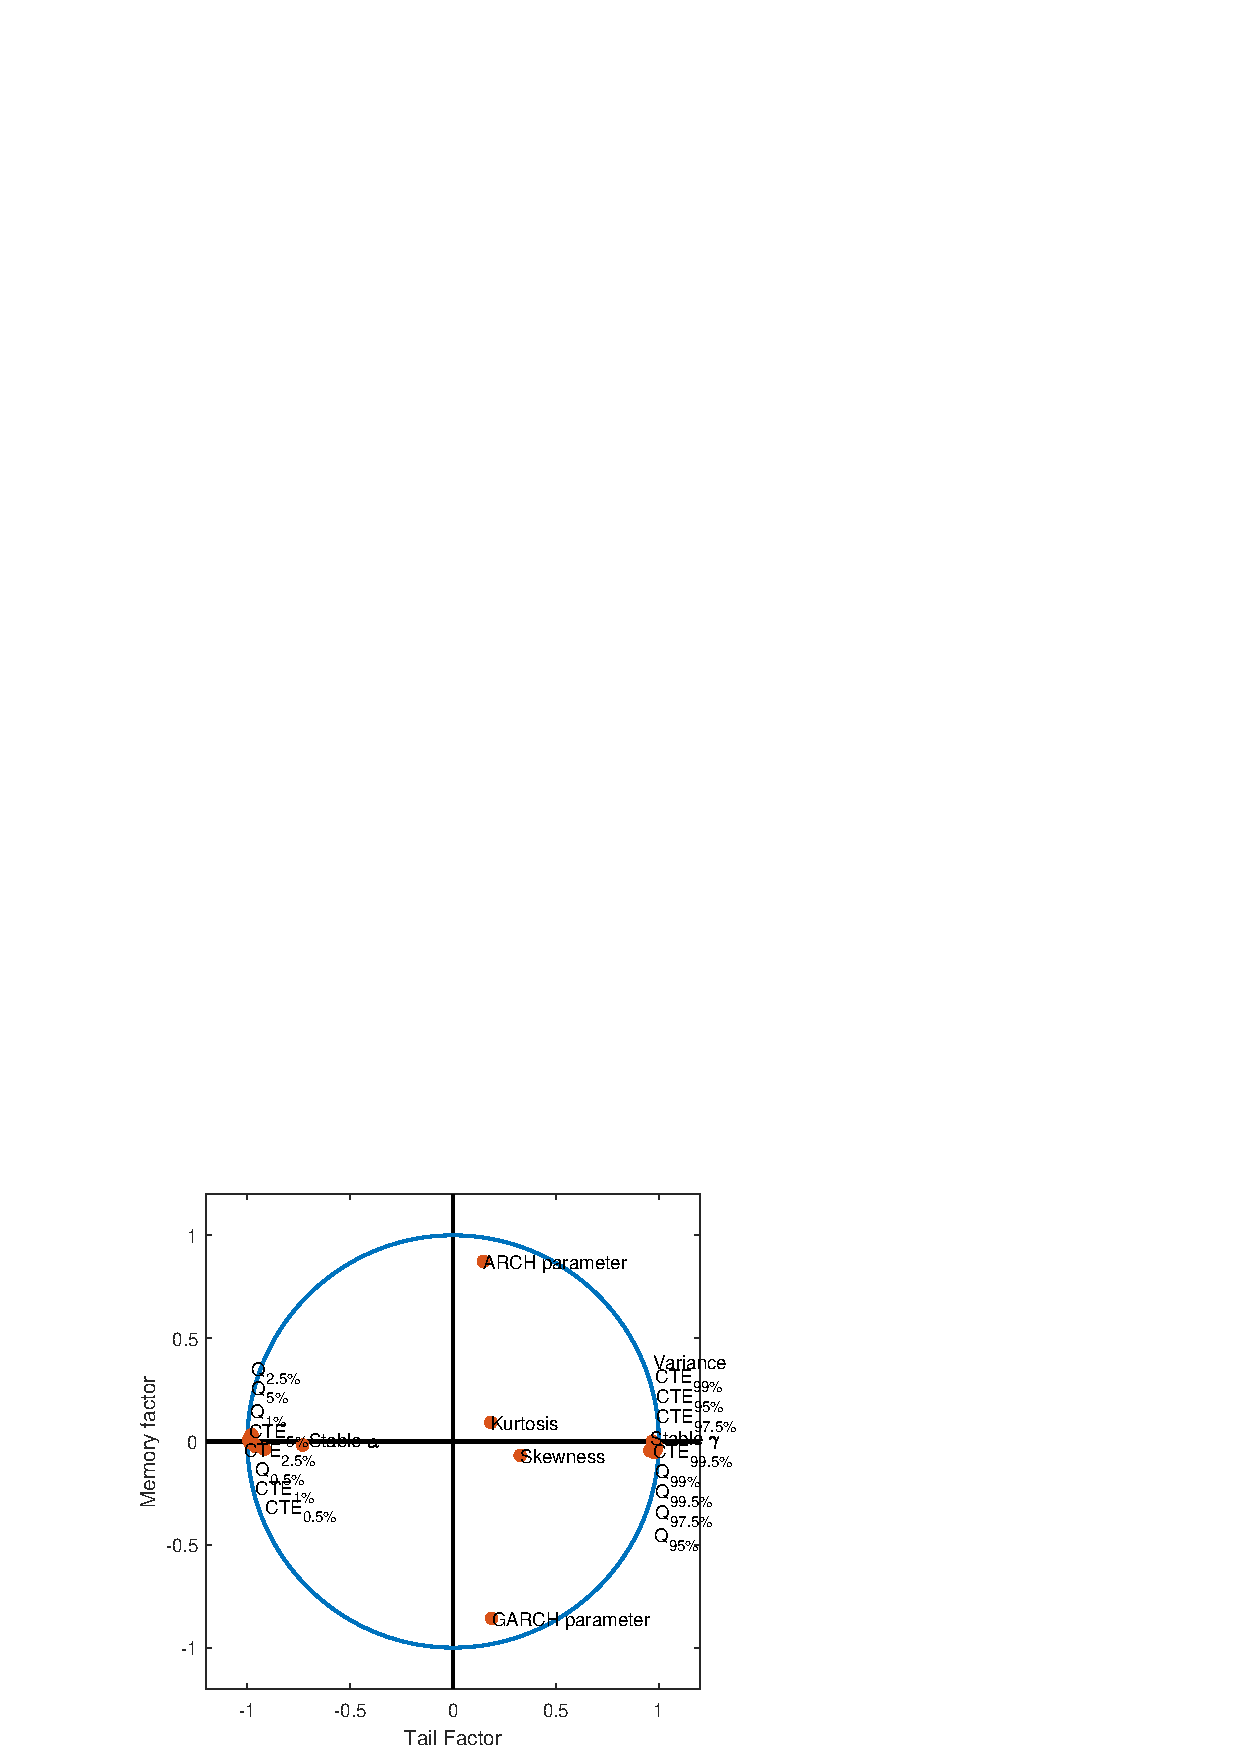
\includegraphics[width=1\textwidth]{Fig/figure_5a}
	
	
\end{minipage}
\begin{minipage}[b]{0.48\textwidth}
	\centering
	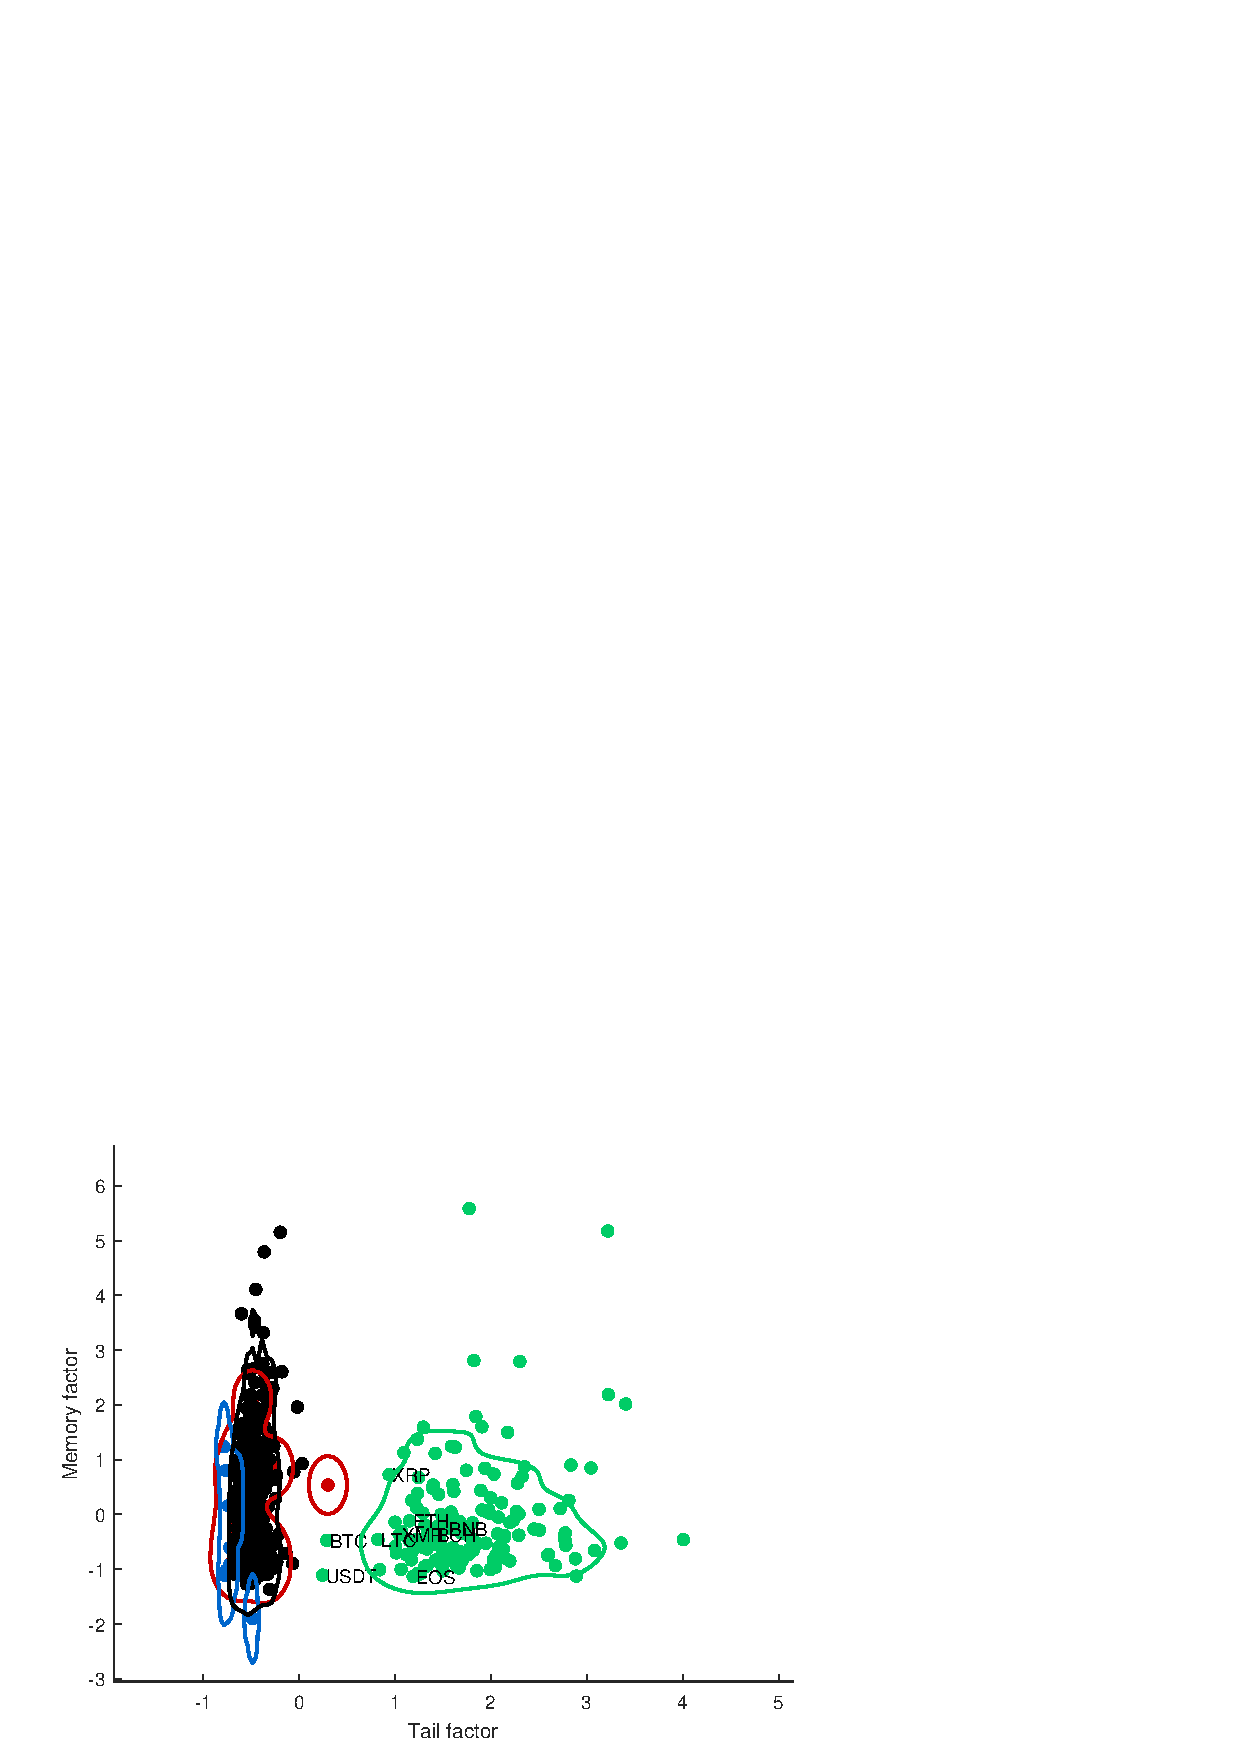
\includegraphics[width=1\textwidth]{Fig/figure_5b}
	
\end{minipage}
\caption {Loadings (left) and scores (right) based on tail and memory factor. \href{https://github.com/QuantLet/Genus_proximum_cryptos/tree/master/SFA_cryptos}{
\includegraphics[width=0.03\textwidth]{Fig/qloqo}\ SFA\_cryptos}}
\end{figure}
}


\frame{
	\frametitle{Moment factor vs Memory factor}
	
	\begin{figure}[!ht]
	\begin{minipage}[b]{0.48\textwidth}
	\centering
	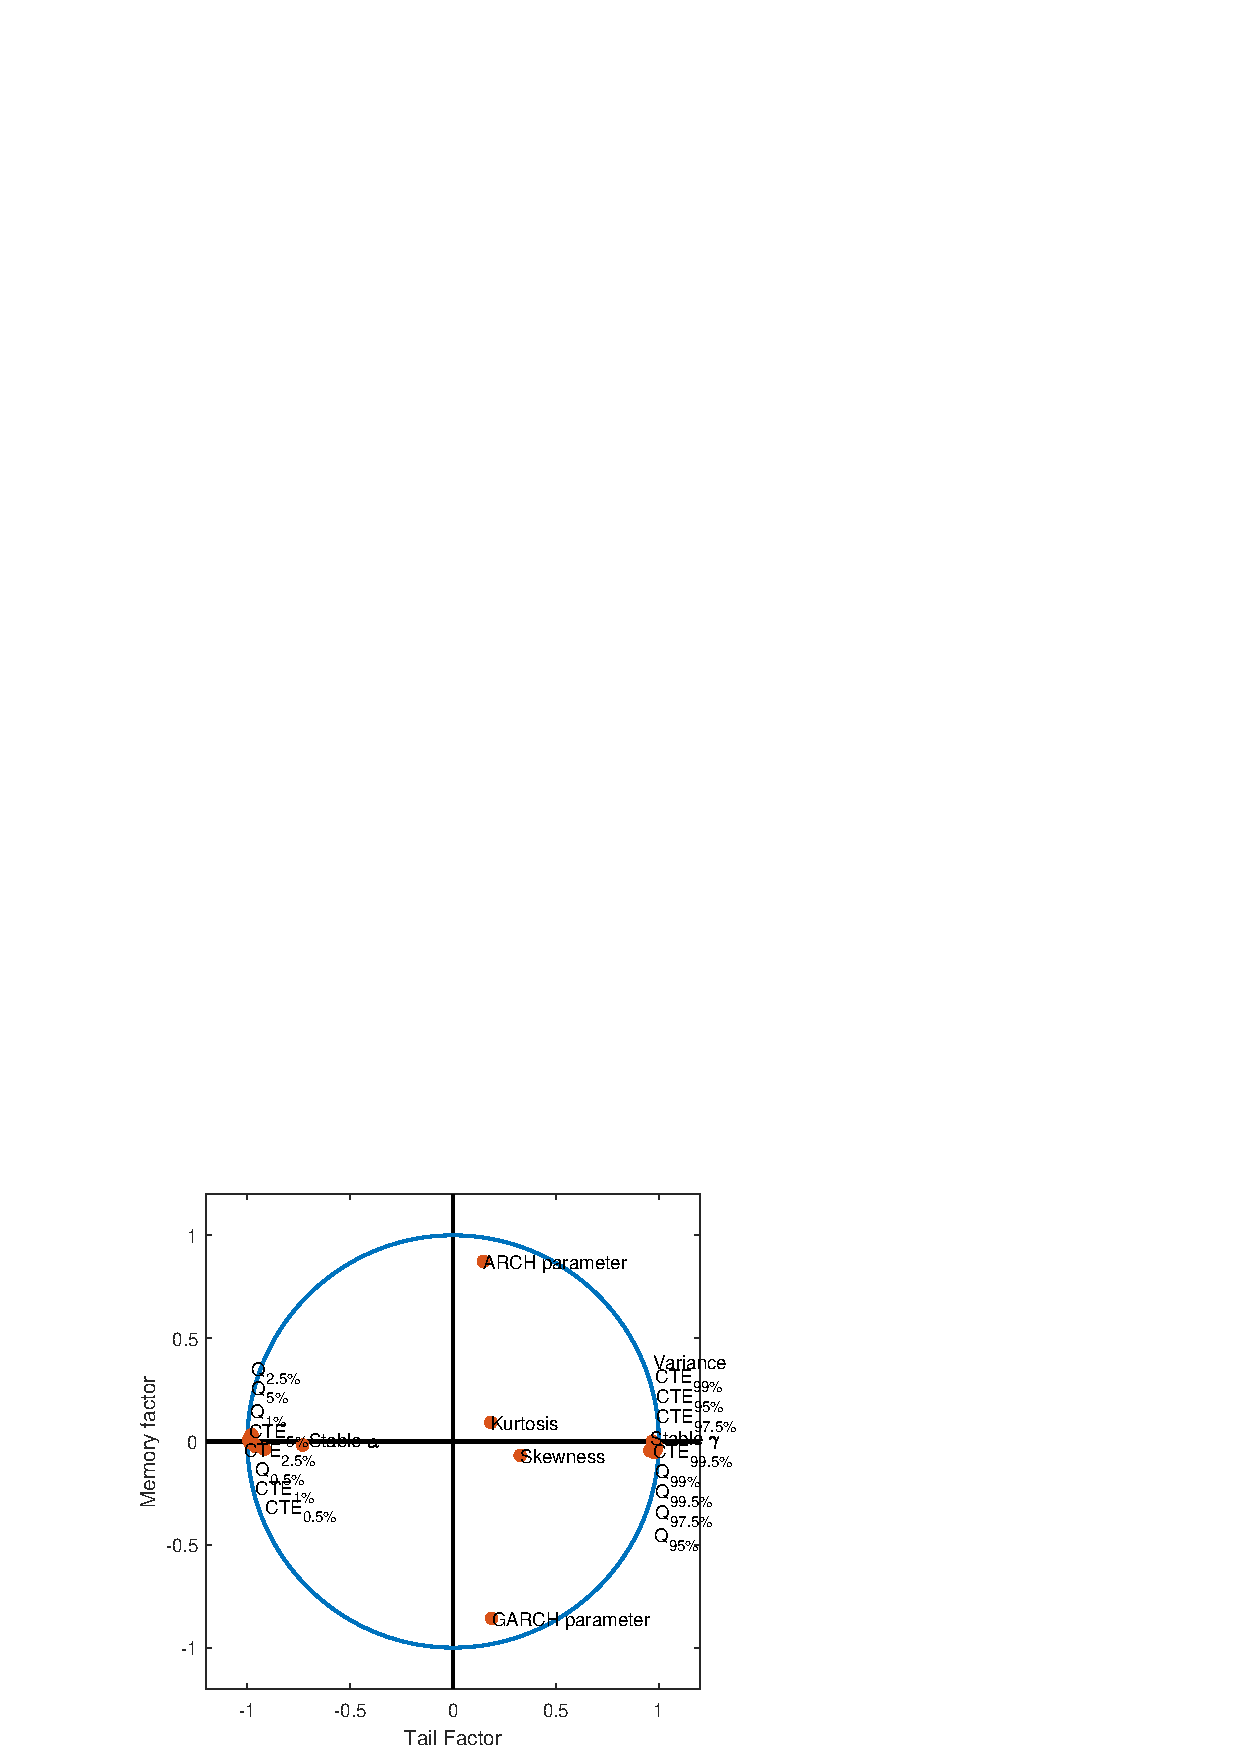
\includegraphics[width=1\textwidth]{Fig/figure_5a}
	
	
\end{minipage}
\begin{minipage}[b]{0.48\textwidth}
	\centering
	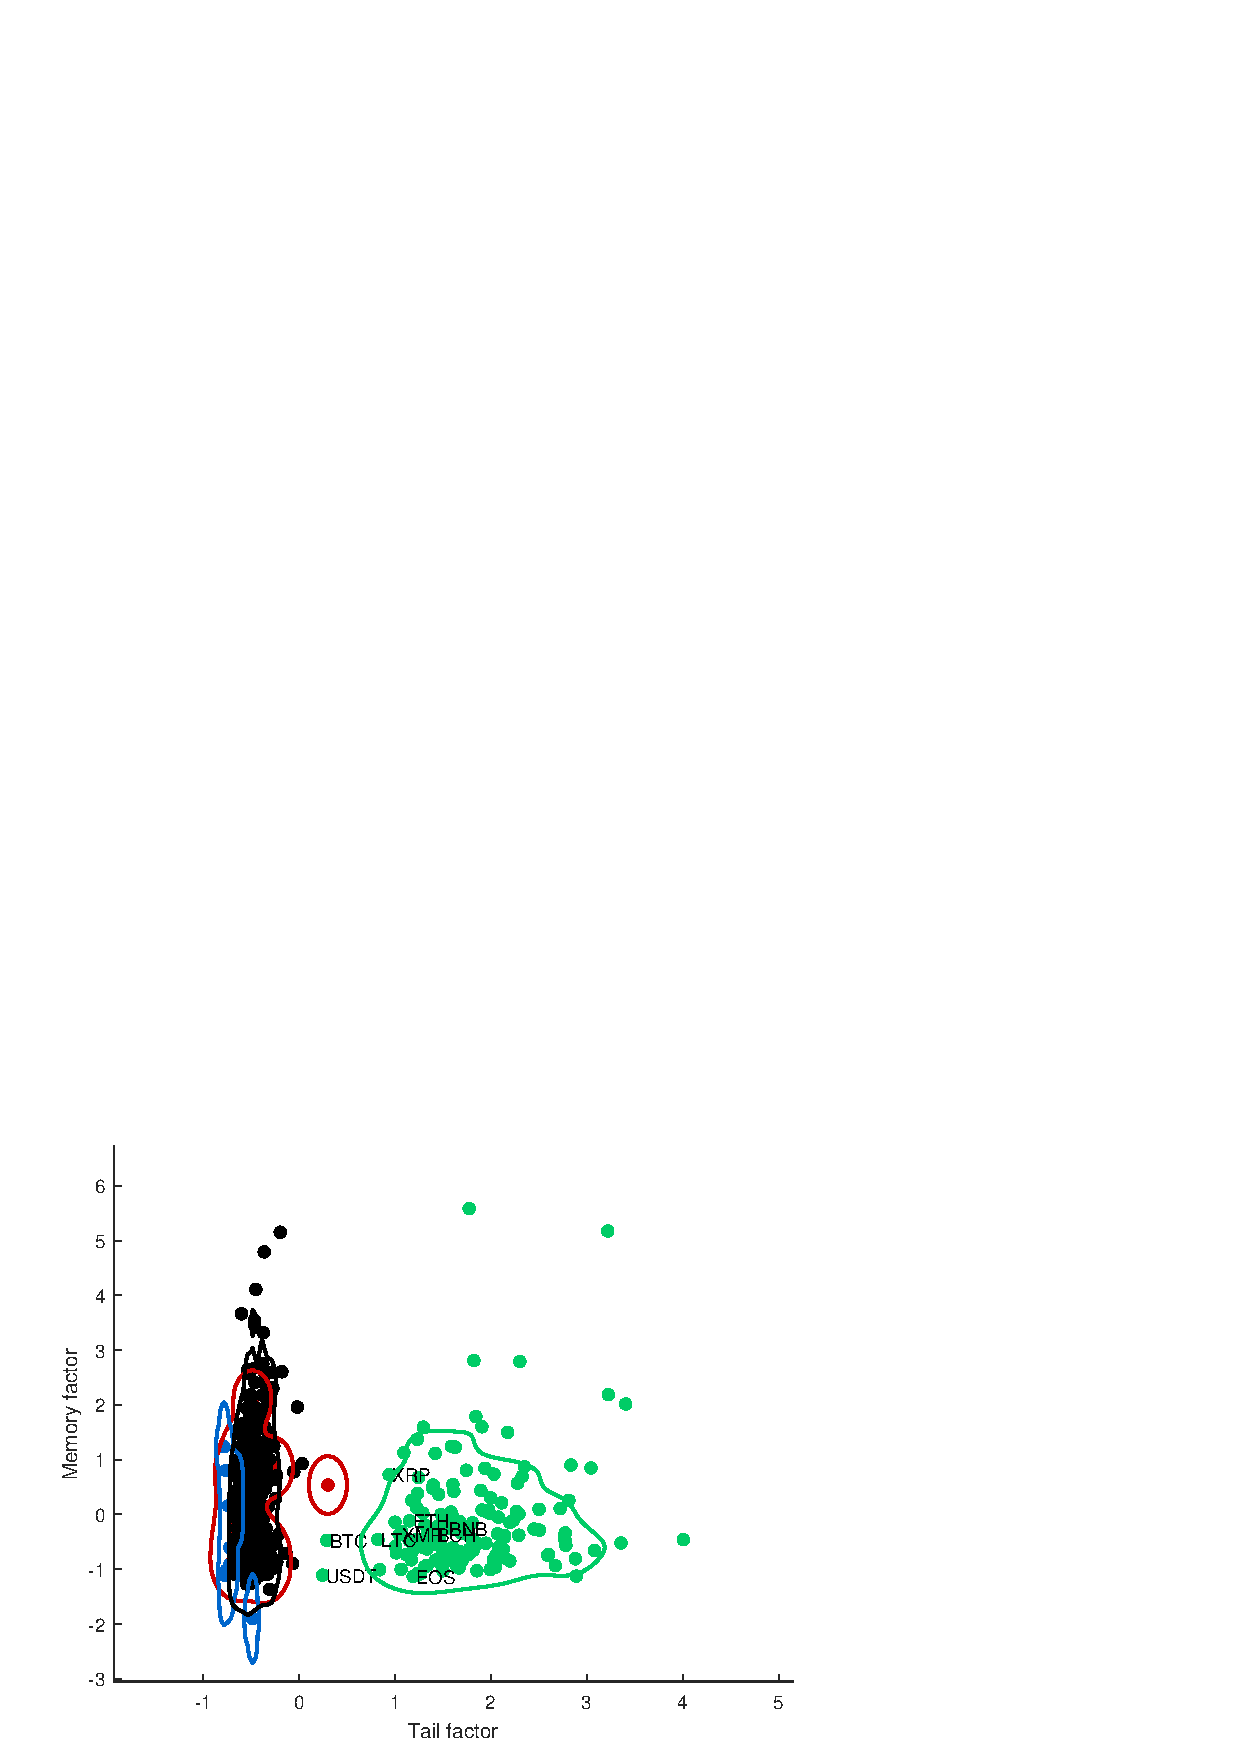
\includegraphics[width=1\textwidth]{Fig/figure_5b}
	
\end{minipage}
\caption {Loadings (left) and scores (right) based on moment and memory factor. \href{https://github.com/QuantLet/Genus_proximum_cryptos/tree/master/SFA_cryptos}{
\includegraphics[width=0.03\textwidth]{Fig/qloqo}\ SFA\_cryptos}}
	\end{figure}
}
%%%%%%%%%%%%%%%%%%%%%%%%%%%%%%%%

\section{Explanation}\label{sec:explanation}

\frame{
\frametitle{Factor explanation}

\begin{itemize}
  \item Classify between Cryptocurrencies and other asset classes
  \item Binary logistic regression for each factor $F_k,\ k\in\left\{1,2,3\right\}$
\end{itemize}

\begin{align}
P(Y=1)=\frac{\exp(\beta_0+\beta_1 F_k)}{1+\exp(\beta_0+\beta_1 F_k)},\\
Y=\begin{cases}
    1, & \text{if Cryptocurrency}\\
    0, & \text{if otherwise}
  \end{cases}
\end{align}

}

\frame{
\frametitle{Factor explanation}

\begin{table}[!ht]
\centering
\small{
	
\begin{tabular}{p{1.5in} p{0.7in} p{0.7in} p{0.7in} } \hline \hline
	\textbf{Exogenous factor} & \textbf{Factor 1} & \textbf{Factor 2} & \textbf{Factor 3} \\ \hline
	Estimated $\beta_{1}$ & 15.679*** & -0.030 & -0.084\\
	& (3.278) & (0.077) & (0.093) \\
	$\tilde{R^2}$  & 0.992 & 0.0003 & 0.002 \\
	\hline \hline
\end{tabular}
\\ 
\tiny {Note: Standard errors in (); ** denotes significance at 95\% confidence level.}
\noindent }

\end{table}

\begin{align}
\tilde{R}^{2}=\frac{1-\left\{\frac{L(\mathbf{0})}{L(\widehat{\boldsymbol{\beta}})}\right\}^{\frac{2}{n}}}{1-\{L(\mathbf{0})\}^{\frac{2}{n}}}
\end{align}
\begin{itemize}
	\item $L(0)$ is the likelihood of the intercept-only model
	\item $L(\widehat{\boldsymbol{\beta}})$ is the likelihood of the full model
\end{itemize}

}


\frame{
\frametitle{Linear Discriminant Analysis} \label{sec:lda}

\begin{minipage}{0.48\textwidth}
\begin{itemize}
  \item Finding a projection that maximizes the separability between classes.
  \item Assumes Gaussianity with equal covariances.
\end{itemize}
\end{minipage}
\hfill
\begin{minipage}{0.48\textwidth}

\begin{figure}[!ht]
\centering
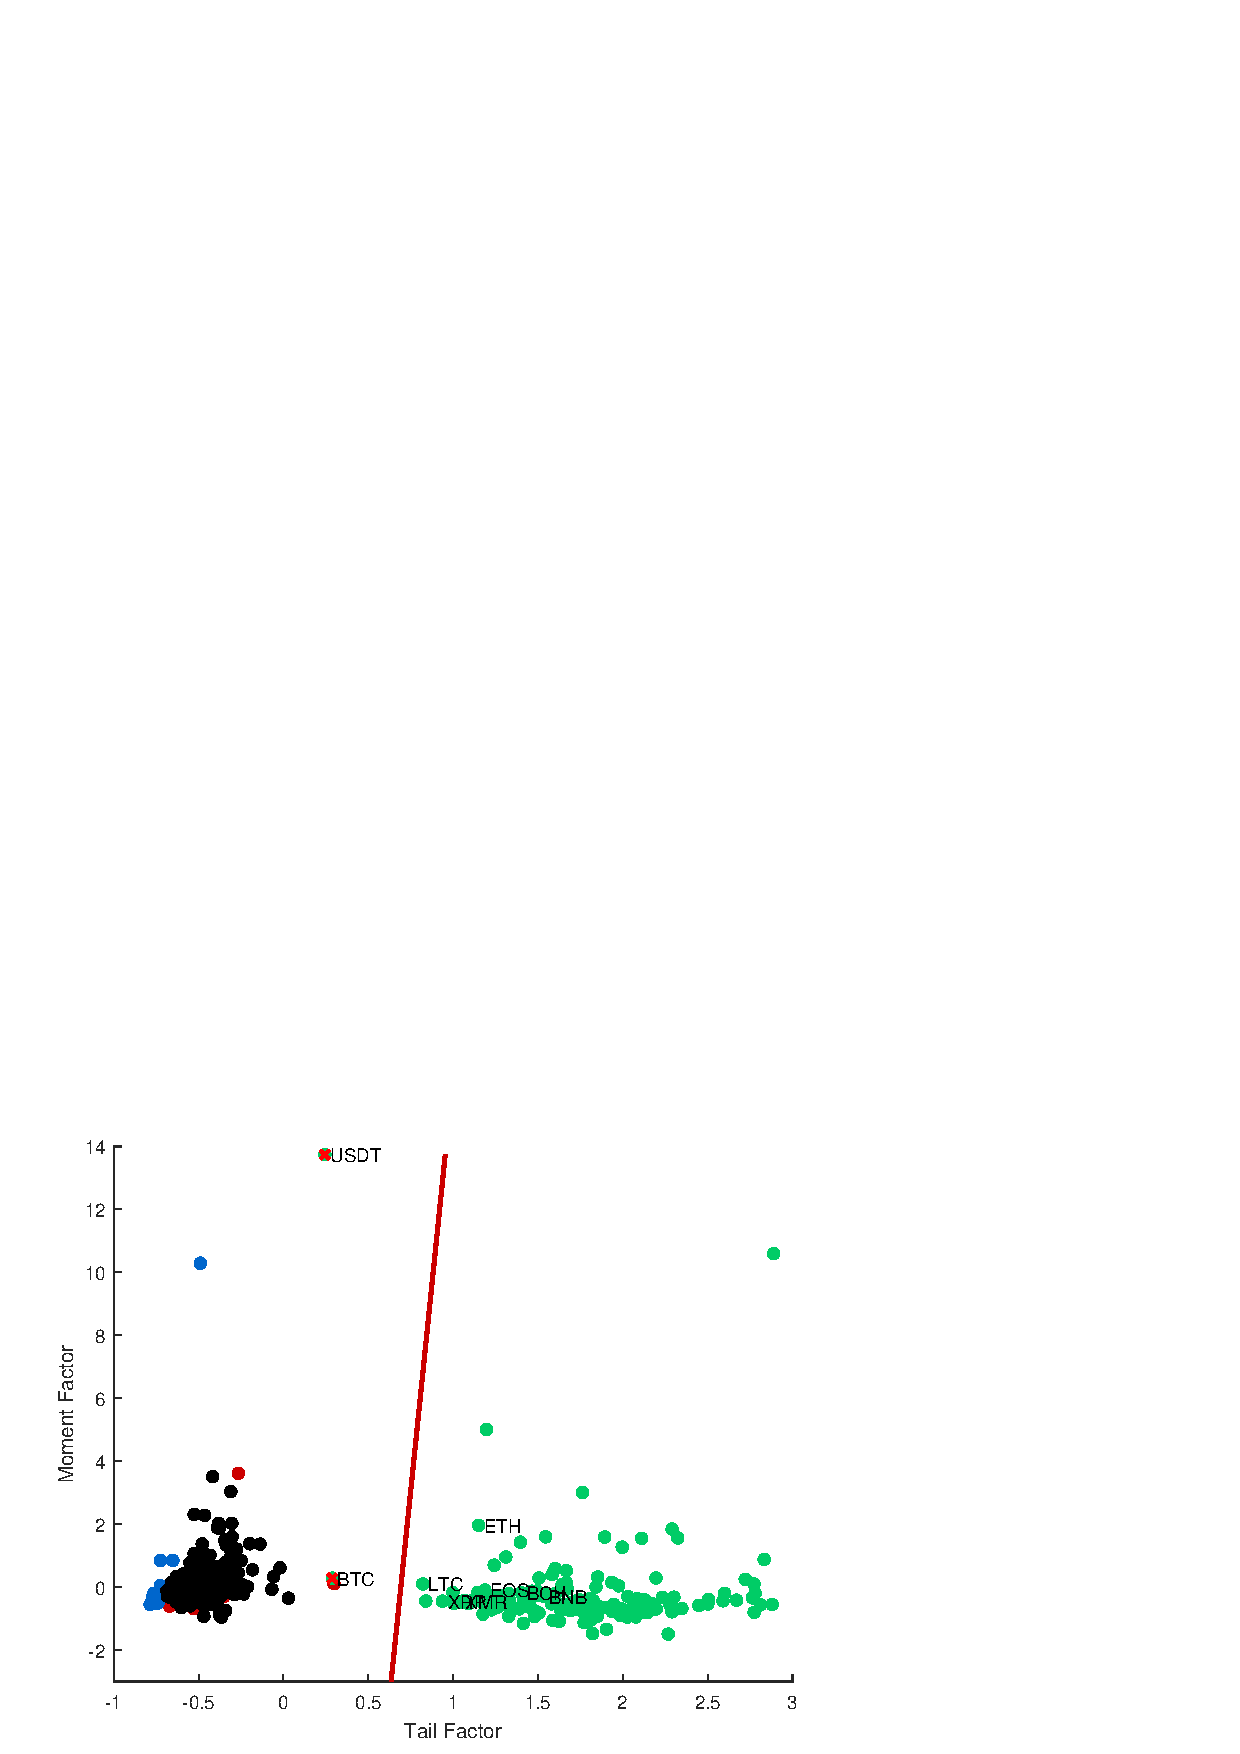
\includegraphics[width=1\textwidth]{Fig/figure_6a}
\caption{LDA \hyperlink{sec:appendix_lda}{\beamergotobutton{LDA}}}
\end{figure}
\end{minipage}
}

\frame{
\frametitle{Quadratic Discriminant Analysis}
\begin{minipage}{0.48\textwidth}
\begin{itemize}
  \item Finding a projection that maximizes the separability between classes.
  \item Assumes Gaussianity with different covariances.
\end{itemize}
\end{minipage}
\hfill
\begin{minipage}{0.48\textwidth}
\begin{figure}[!ht]
\centering
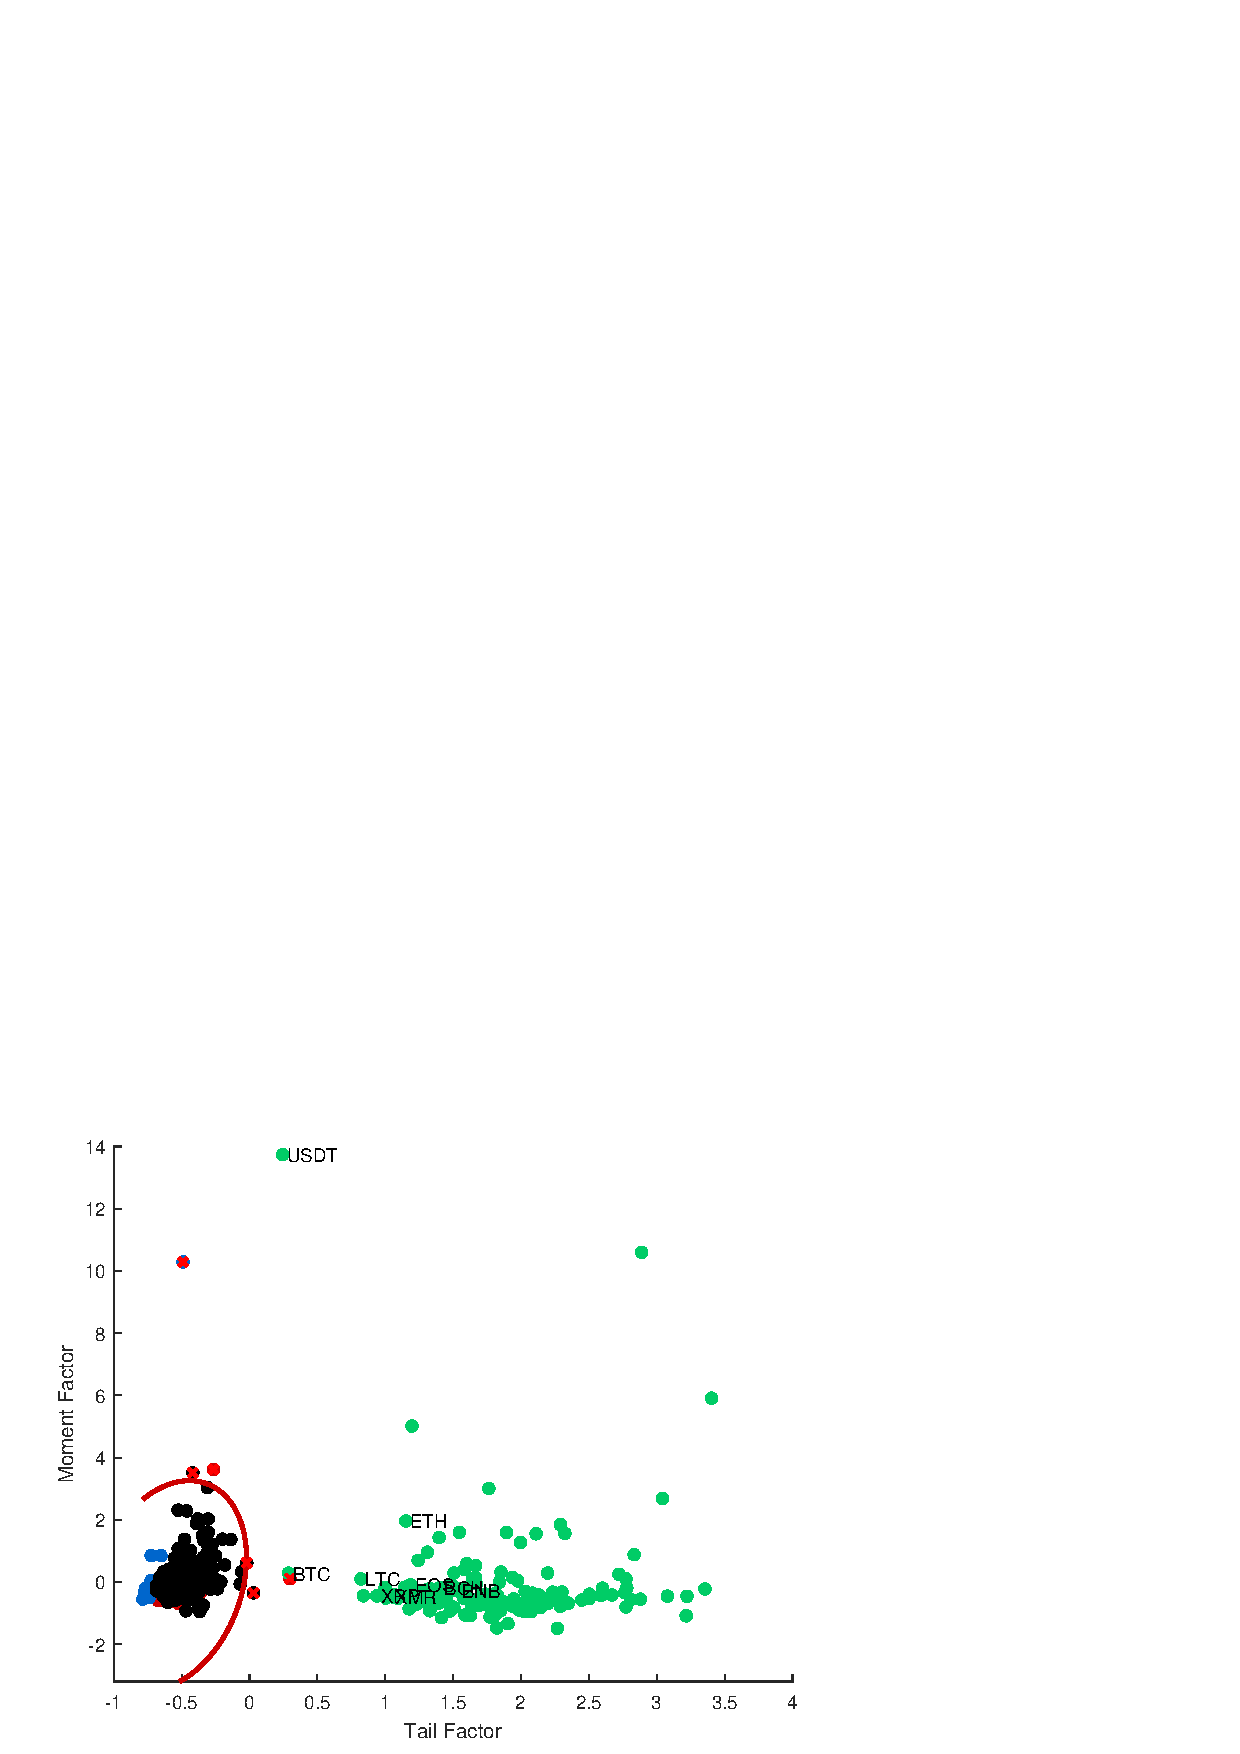
\includegraphics[width=1\textwidth]{Fig/figure_6b}
\caption{Quadratic Discriminant Analysis}
\end{figure}
\end{minipage}
}
%%%%%%%%%%%%%%%%%%%%%%%%%%%%%%%%
\frame{
\frametitle{Support Vector Machines} \label{sec:svm}
\begin{minipage}{0.48\textwidth}
\begin{itemize}
  \item Finding a projection that maximizes margin in a hyperplane of the original data.
  \item No parametric assumptions on the underlying probability distribution function.
\end{itemize}
\end{minipage}
\hfill
\begin{minipage}{0.48\textwidth}
\begin{figure}[!ht]
\centering
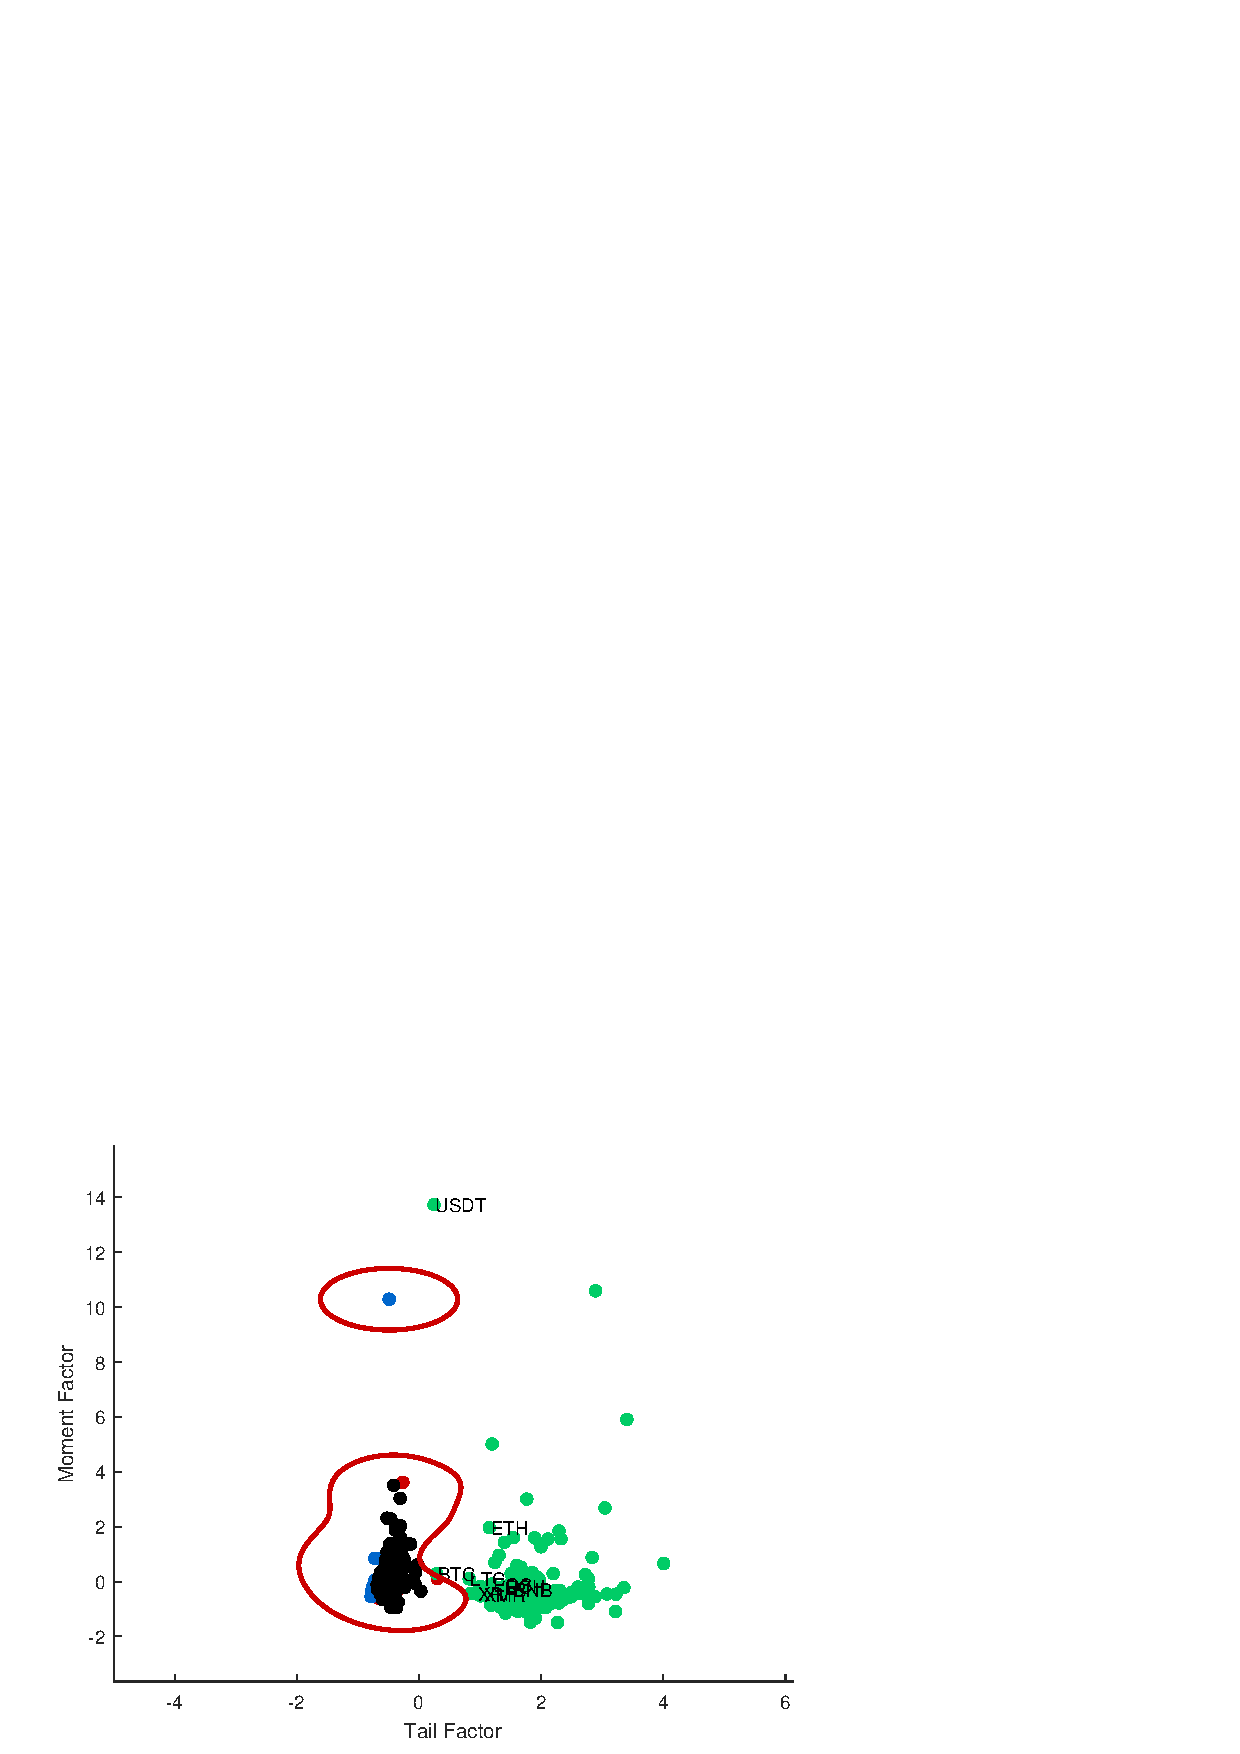
\includegraphics[width=1\textwidth]{Fig/figure_7}
\caption{SVM \hyperlink{sec:appendix_svm}{\beamergotobutton{SVM}}}
\end{figure}
\end{minipage}
}

\frame{
	\frametitle{K-means clustering} \label{sec:kms}
	\begin{minipage}{0.48\textwidth}
		\begin{itemize}
			\item Projection of the clusters on the 3D space extracted trough Factor Analysis.
			\item Each cryptocurrencies cluster was labeled with its leader in terms of market capitalization.
		\end{itemize}
	\end{minipage}
	\hfill
	\begin{minipage}{0.48\textwidth}
		\begin{figure}[!ht]
			\centering
			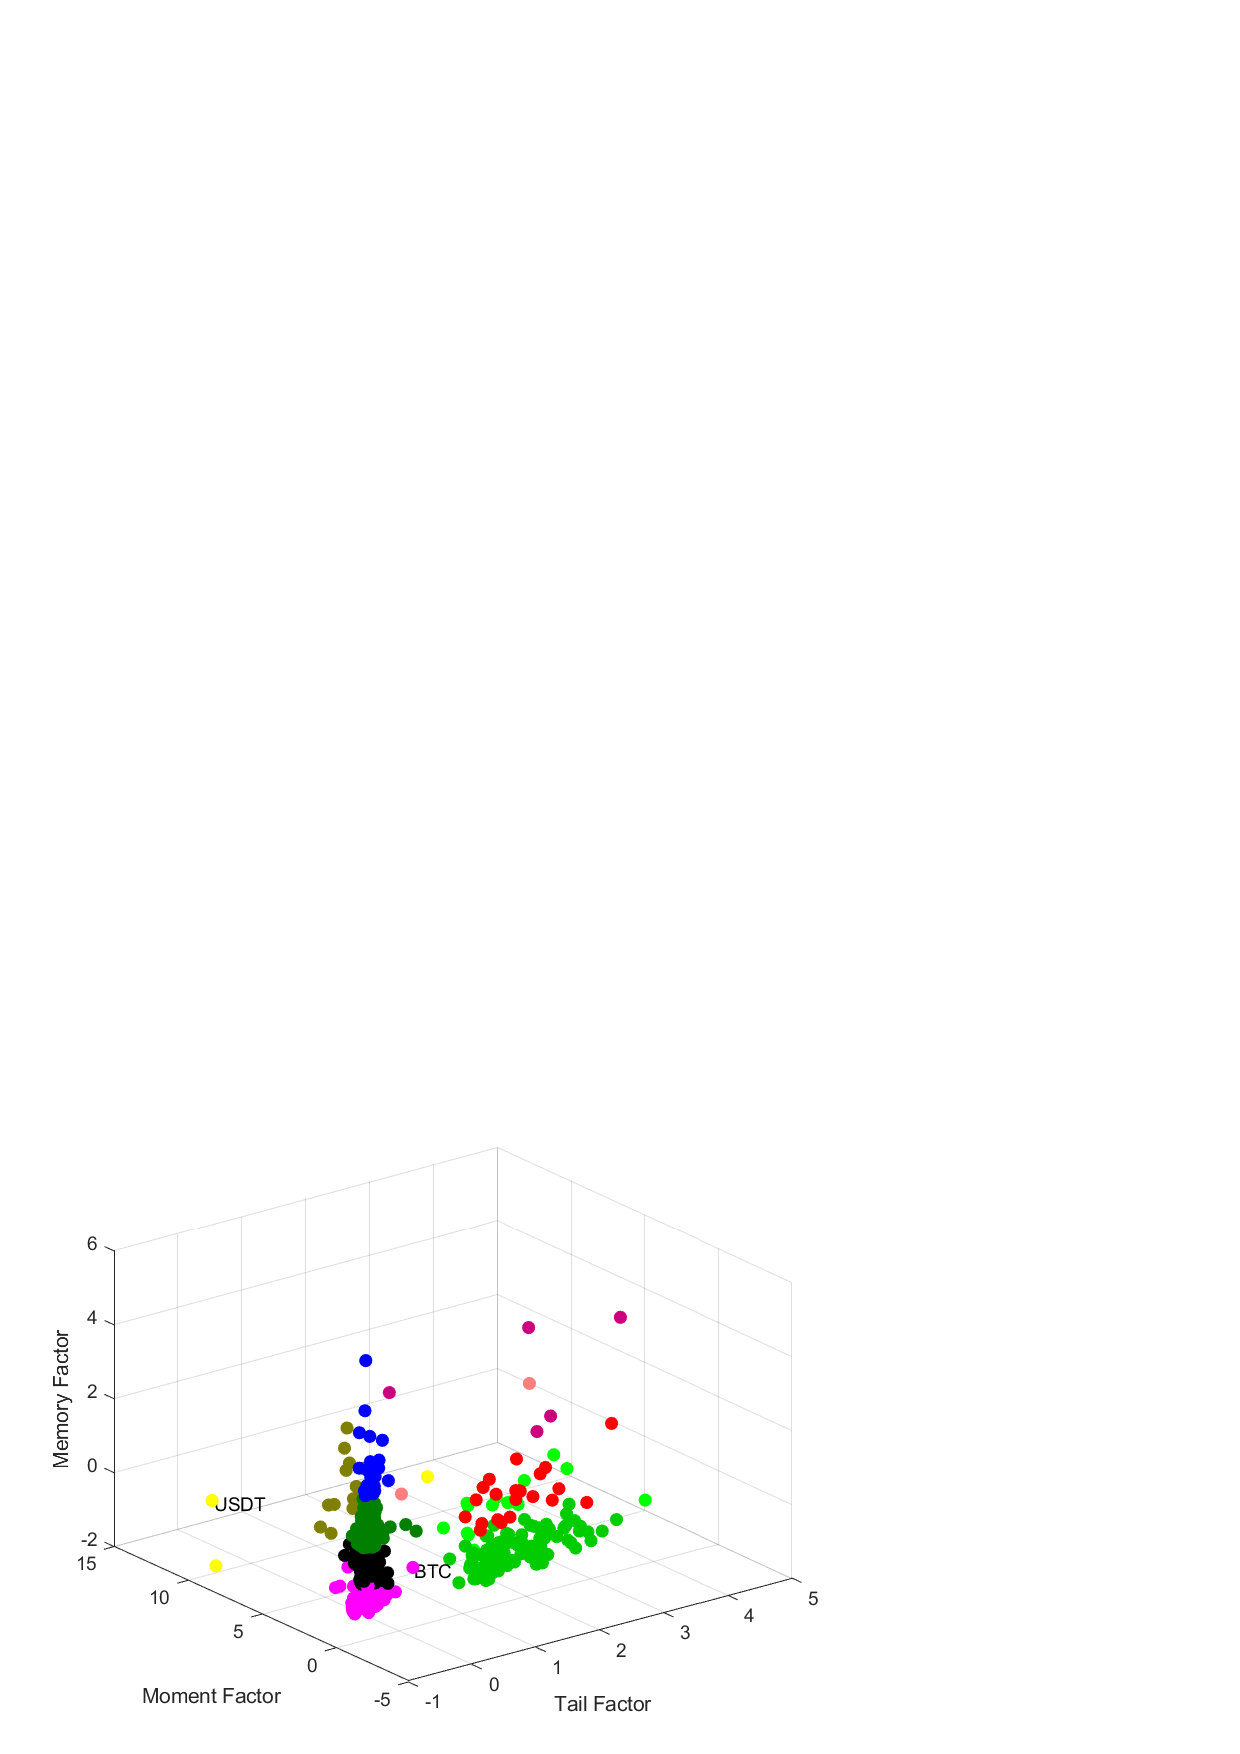
\includegraphics[width=1\textwidth]{Fig/figure_8}
			\caption{\centering 3D. \href{https://github.com/QuantLet/Genus_proximum_cryptos/tree/master/Cluster_cryptos}{
\includegraphics[width=0.05\textwidth]{Fig/qloqo}\ Cluster\_cryptos}}
		\end{figure}
	\end{minipage}
}

\frame{
	\frametitle{Maximum Variance Components Split} \label{sec:MVCS}
	\begin{minipage}{0.5\textwidth}
		\begin{itemize}
			\item These method have goals to separate, respectively, the components of a structure like the types of assets herein, and clusters defined as the components of a mixture distribution.
			\item They are based on an unusual variance decomposition in between-group variations.
		\end{itemize}
	\end{minipage}
	\hfill
	\begin{minipage}{0.48\textwidth}
\begin{figure}[!ht]
	\centering
	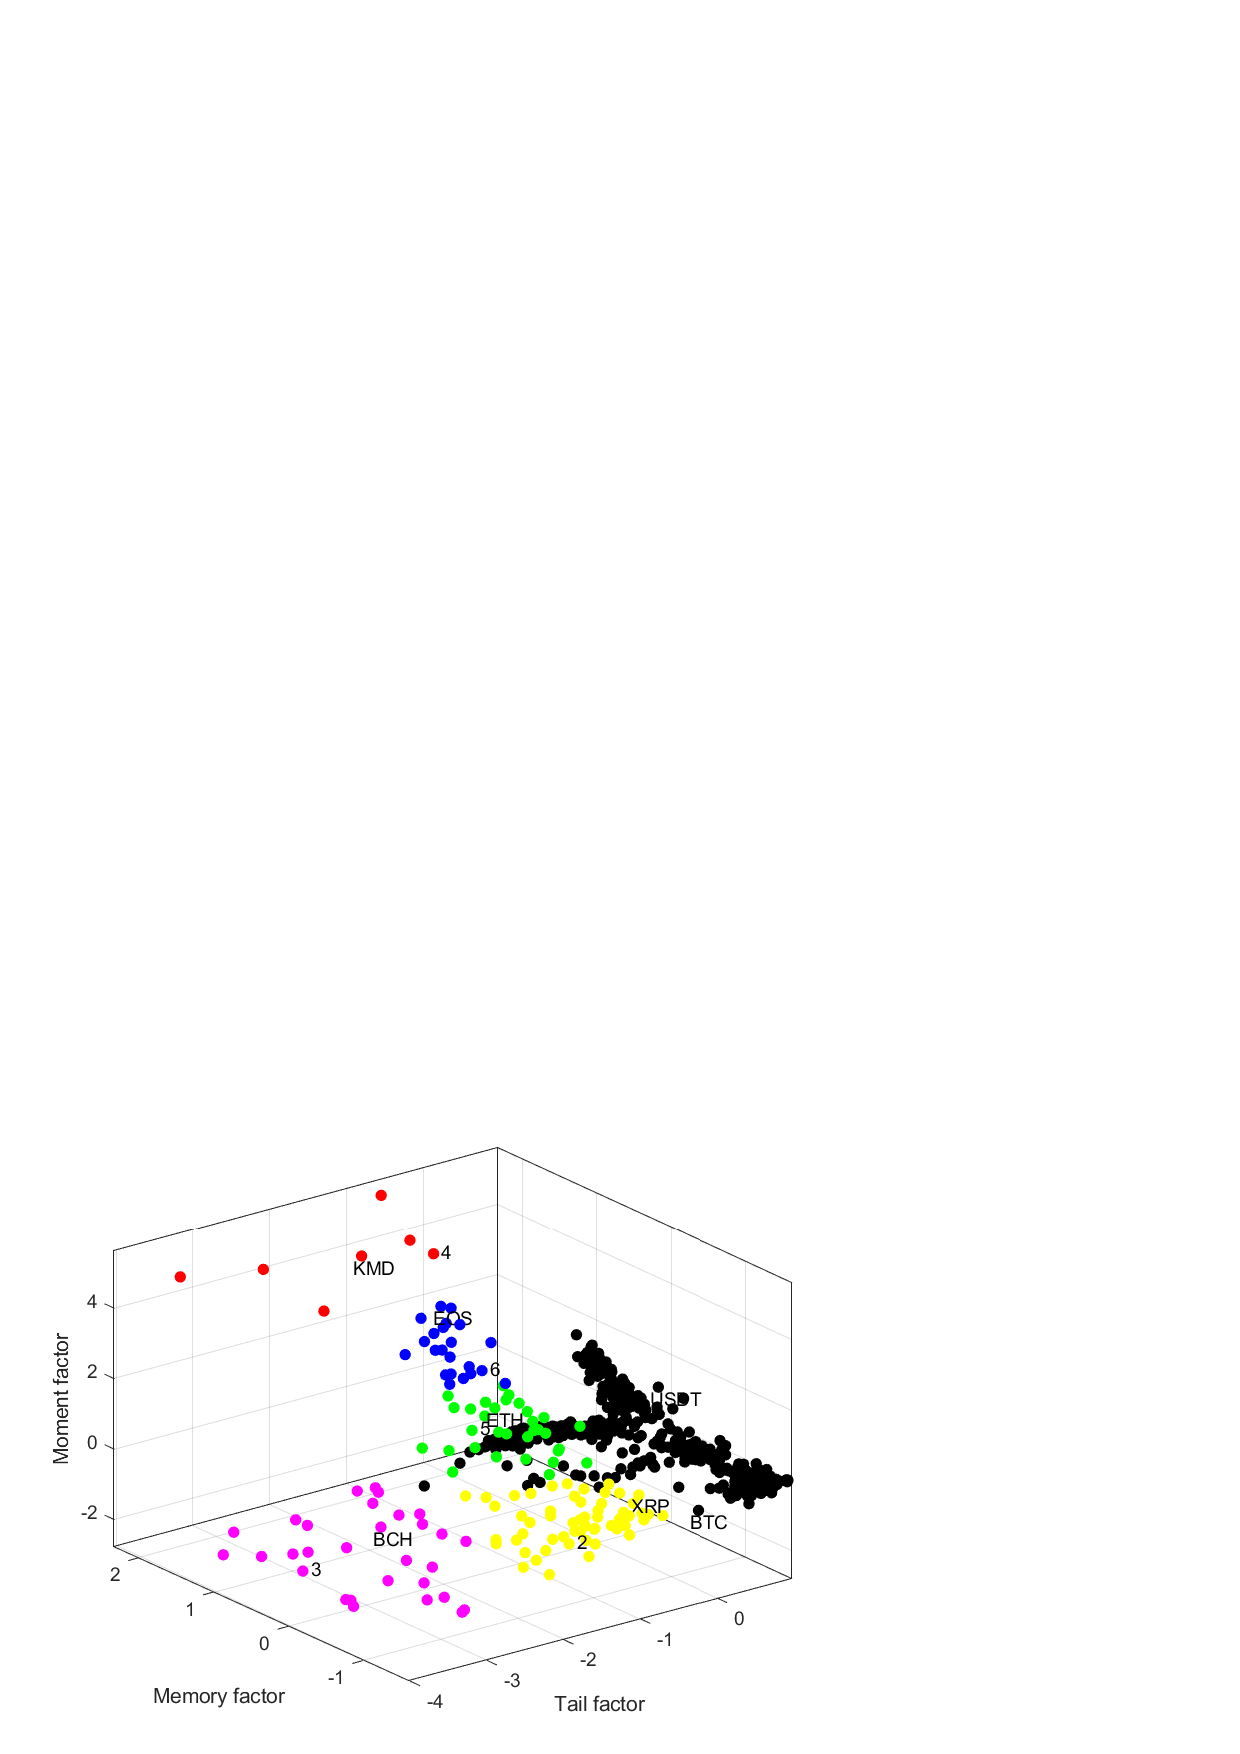
\includegraphics[width=1.25\textwidth]{Fig/figure_9}
	\caption{\centering MVCS. \href{https://github.com/QuantLet/Genus_proximum_cryptos/tree/master/VCS_cryptos}{
\includegraphics[width=0.05\textwidth]{Fig/qloqo}\ VCS\_cryptos} \hyperlink{sec:appendix_MVCS}{\beamergotobutton{MVCS}}}
	\label{fig:figure_10}
\end{figure}
	\end{minipage}

}

%%%%%%%%%%%%%%%%%%%%%%%%%%%%%%%%

%%%%%%%%%%%%%%%%%%%%%%%%%%%%%%%%

\section{Video}

\frame{
\frametitle{Video}

\begin{itemize}
  \item Expanding rolling window estimation
  \begin{itemize}
    \item Starting window 2014-01-02 until 2016-10-231 ($1/2$ of the data)
    \item Increases daily up to full window 2014-01-02 until 2019-08-30
    \item Kernel density contour level $0.015$
  \end{itemize}
  \item Clusters converge over time
\end{itemize}

\begin{figure}
    \centering
    \href{Fig/crypto-movie.mp4}{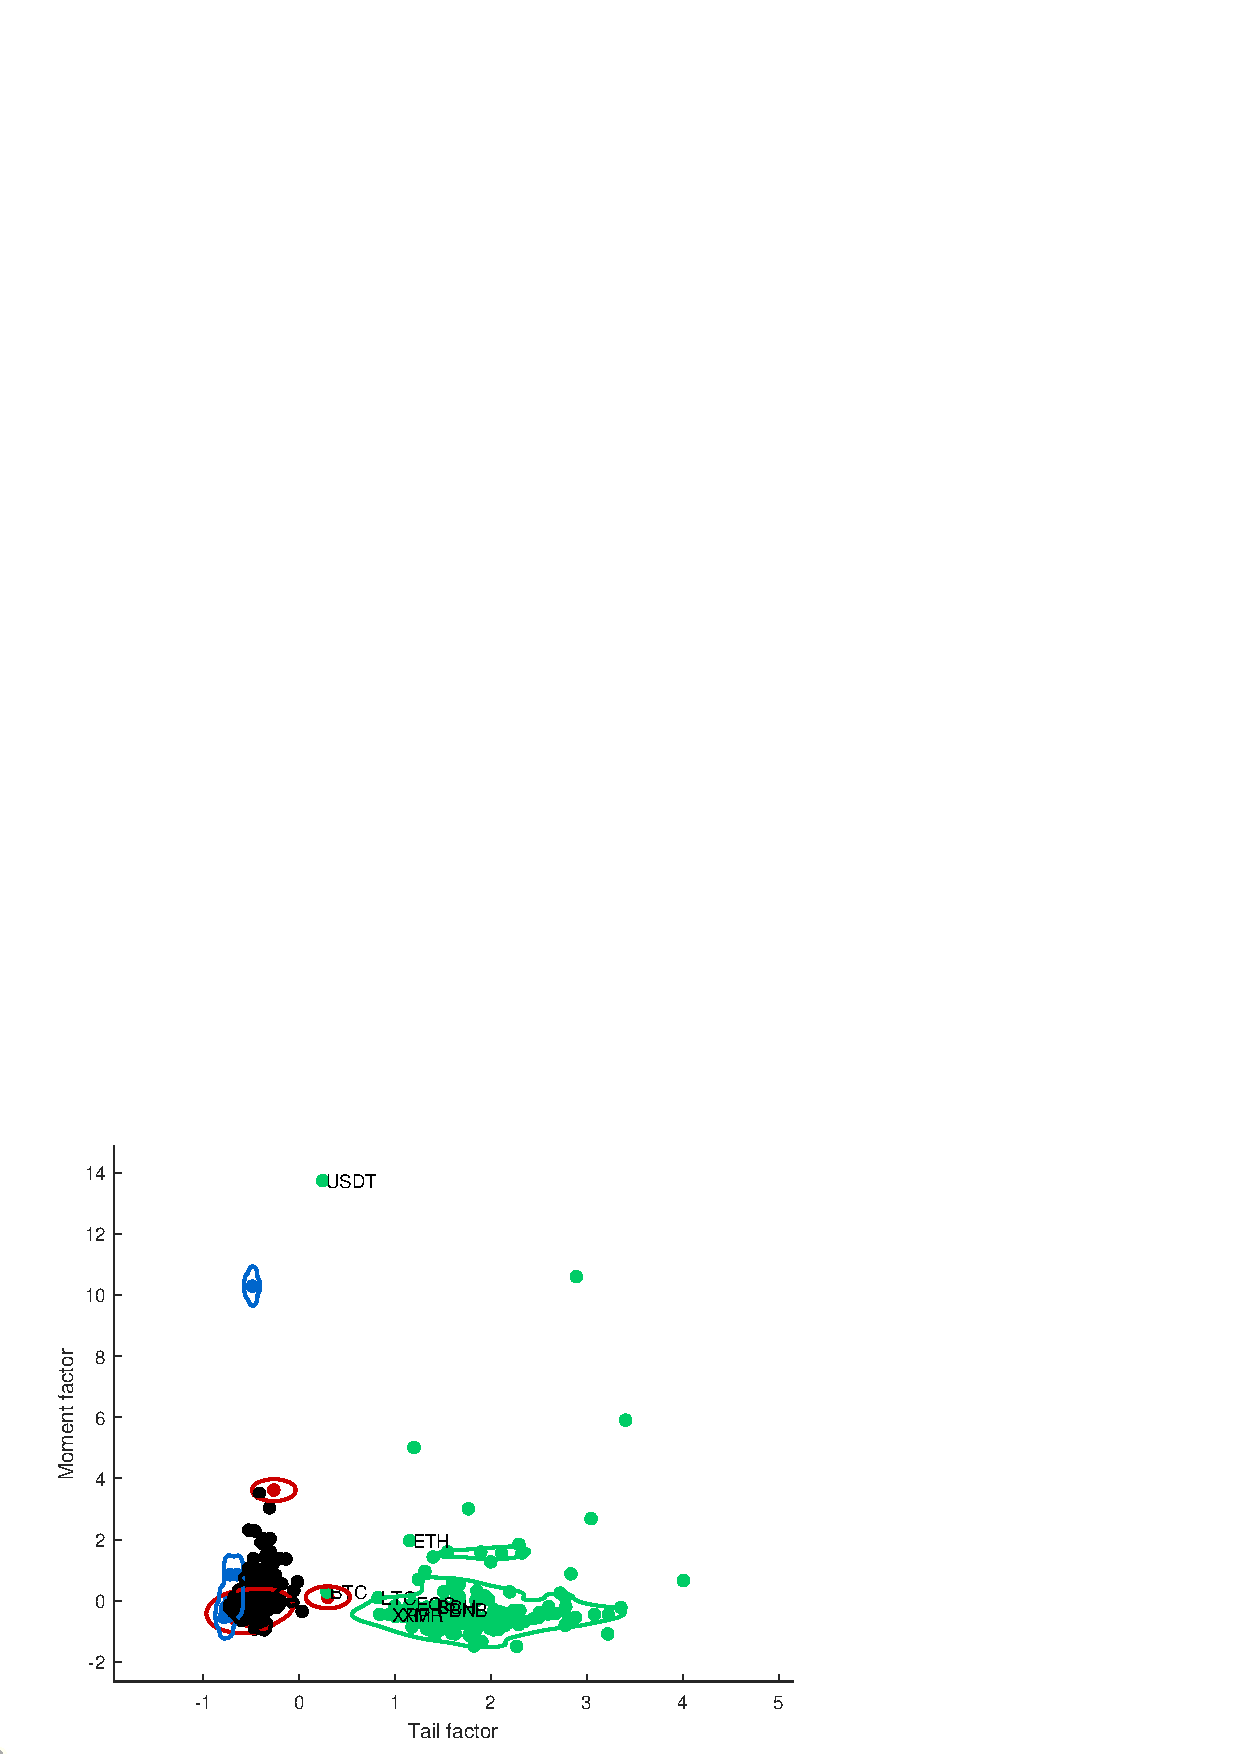
\includegraphics[width=0.4\textwidth]{Fig/figure_4b}}

\end{figure}
   \centering
\href{https://github.com/QuantLet/Genus_proximum_cryptos/tree/master/DFA_cryptos}{
\includegraphics[width=0.03\textwidth]{Fig/qloqo}\ DFA\_cryptos}
}

\frame{
	\frametitle{Synchronic evolution}
	
	\begin{figure}[!ht]
	\centering
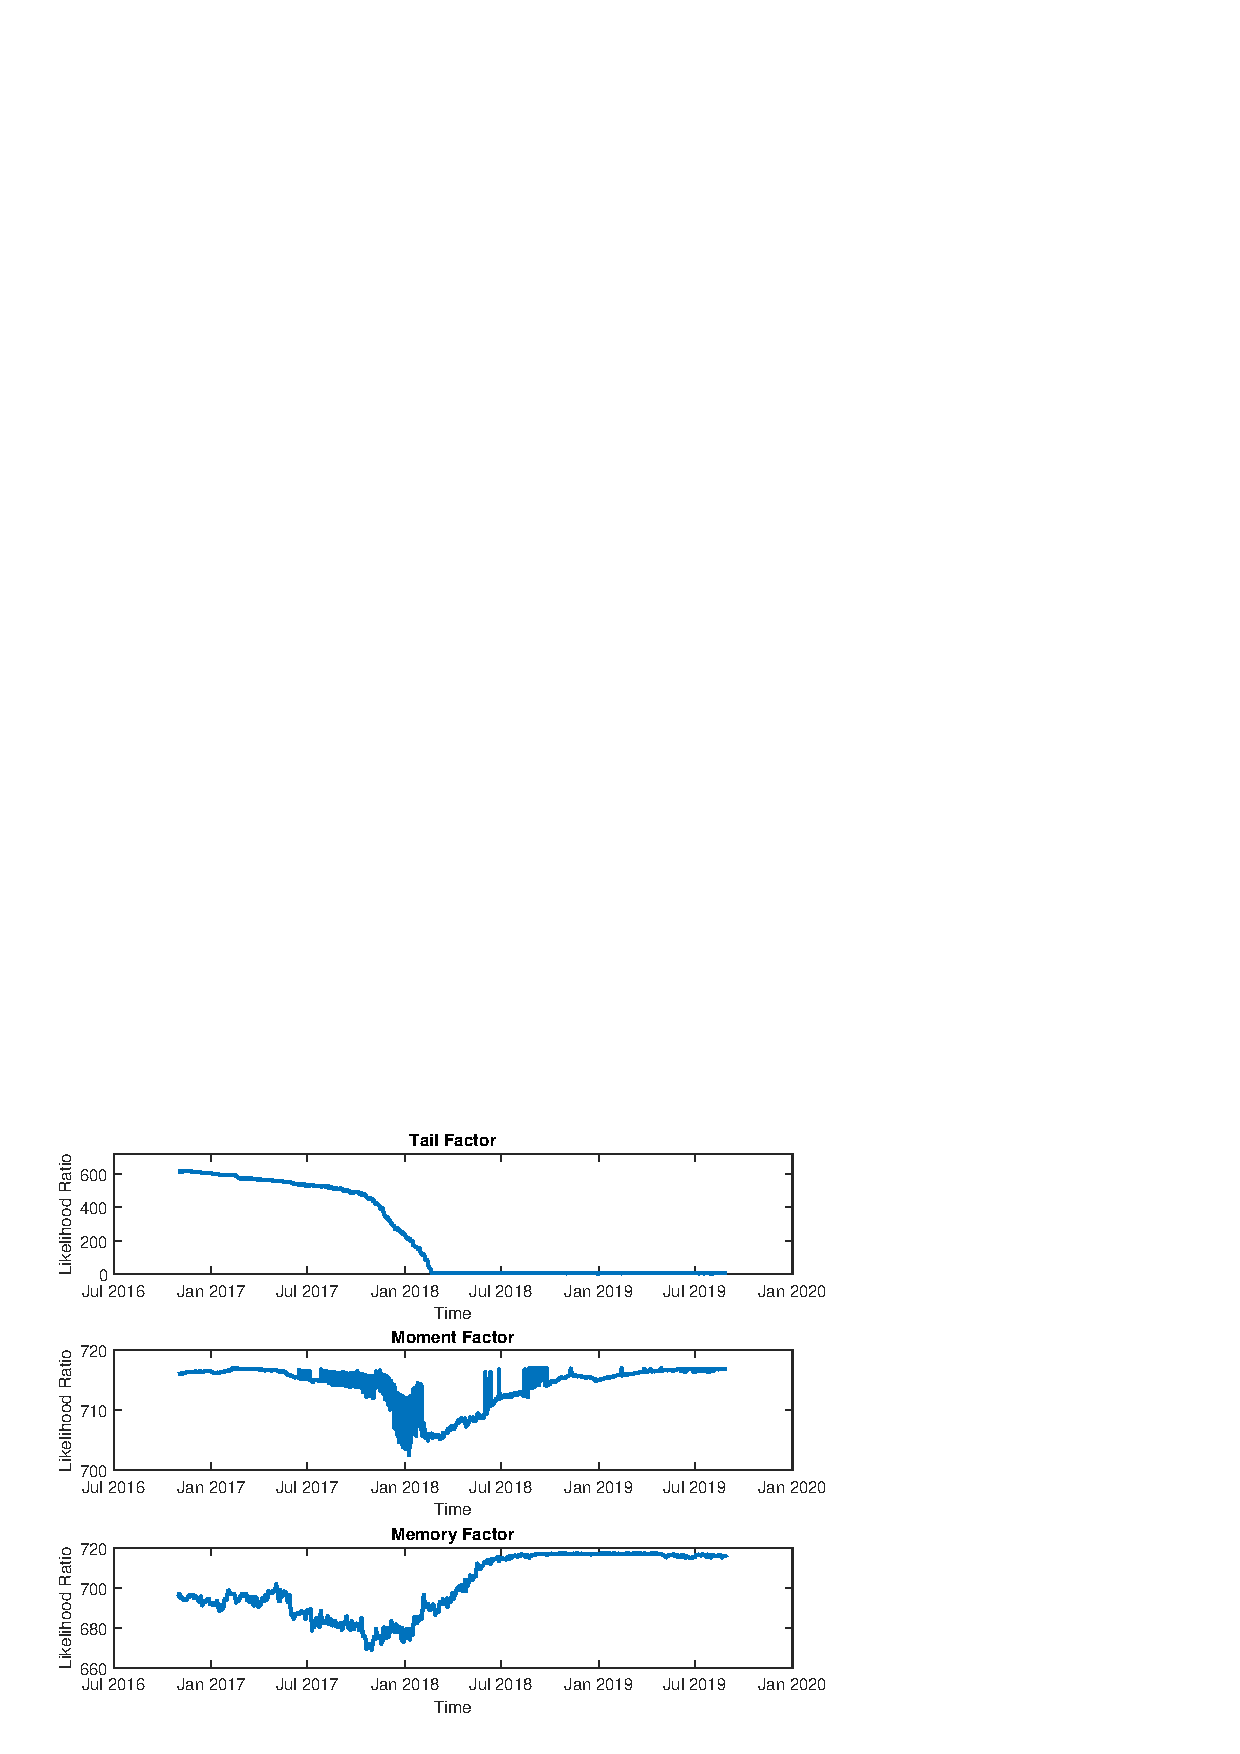
\includegraphics[width=0.7\textwidth]{Fig/figure_12}
\caption{Likelihood Ratios for the binary logistic model, estimated for the period 10/31/2016-
	08/30/2019.\href{https://github.com/QuantLet/Genus_proximum_cryptos/tree/master/CONV_cryptos}{
\includegraphics[width=0.03\textwidth]{Fig/qloqo}\ CONV\_cryptos}}
	\end{figure}
}

\section{Conclusion}
%\frame{
%\frametitle{Cryptocurrencies profile}
%\begin{figure}[!profile]
%	
%	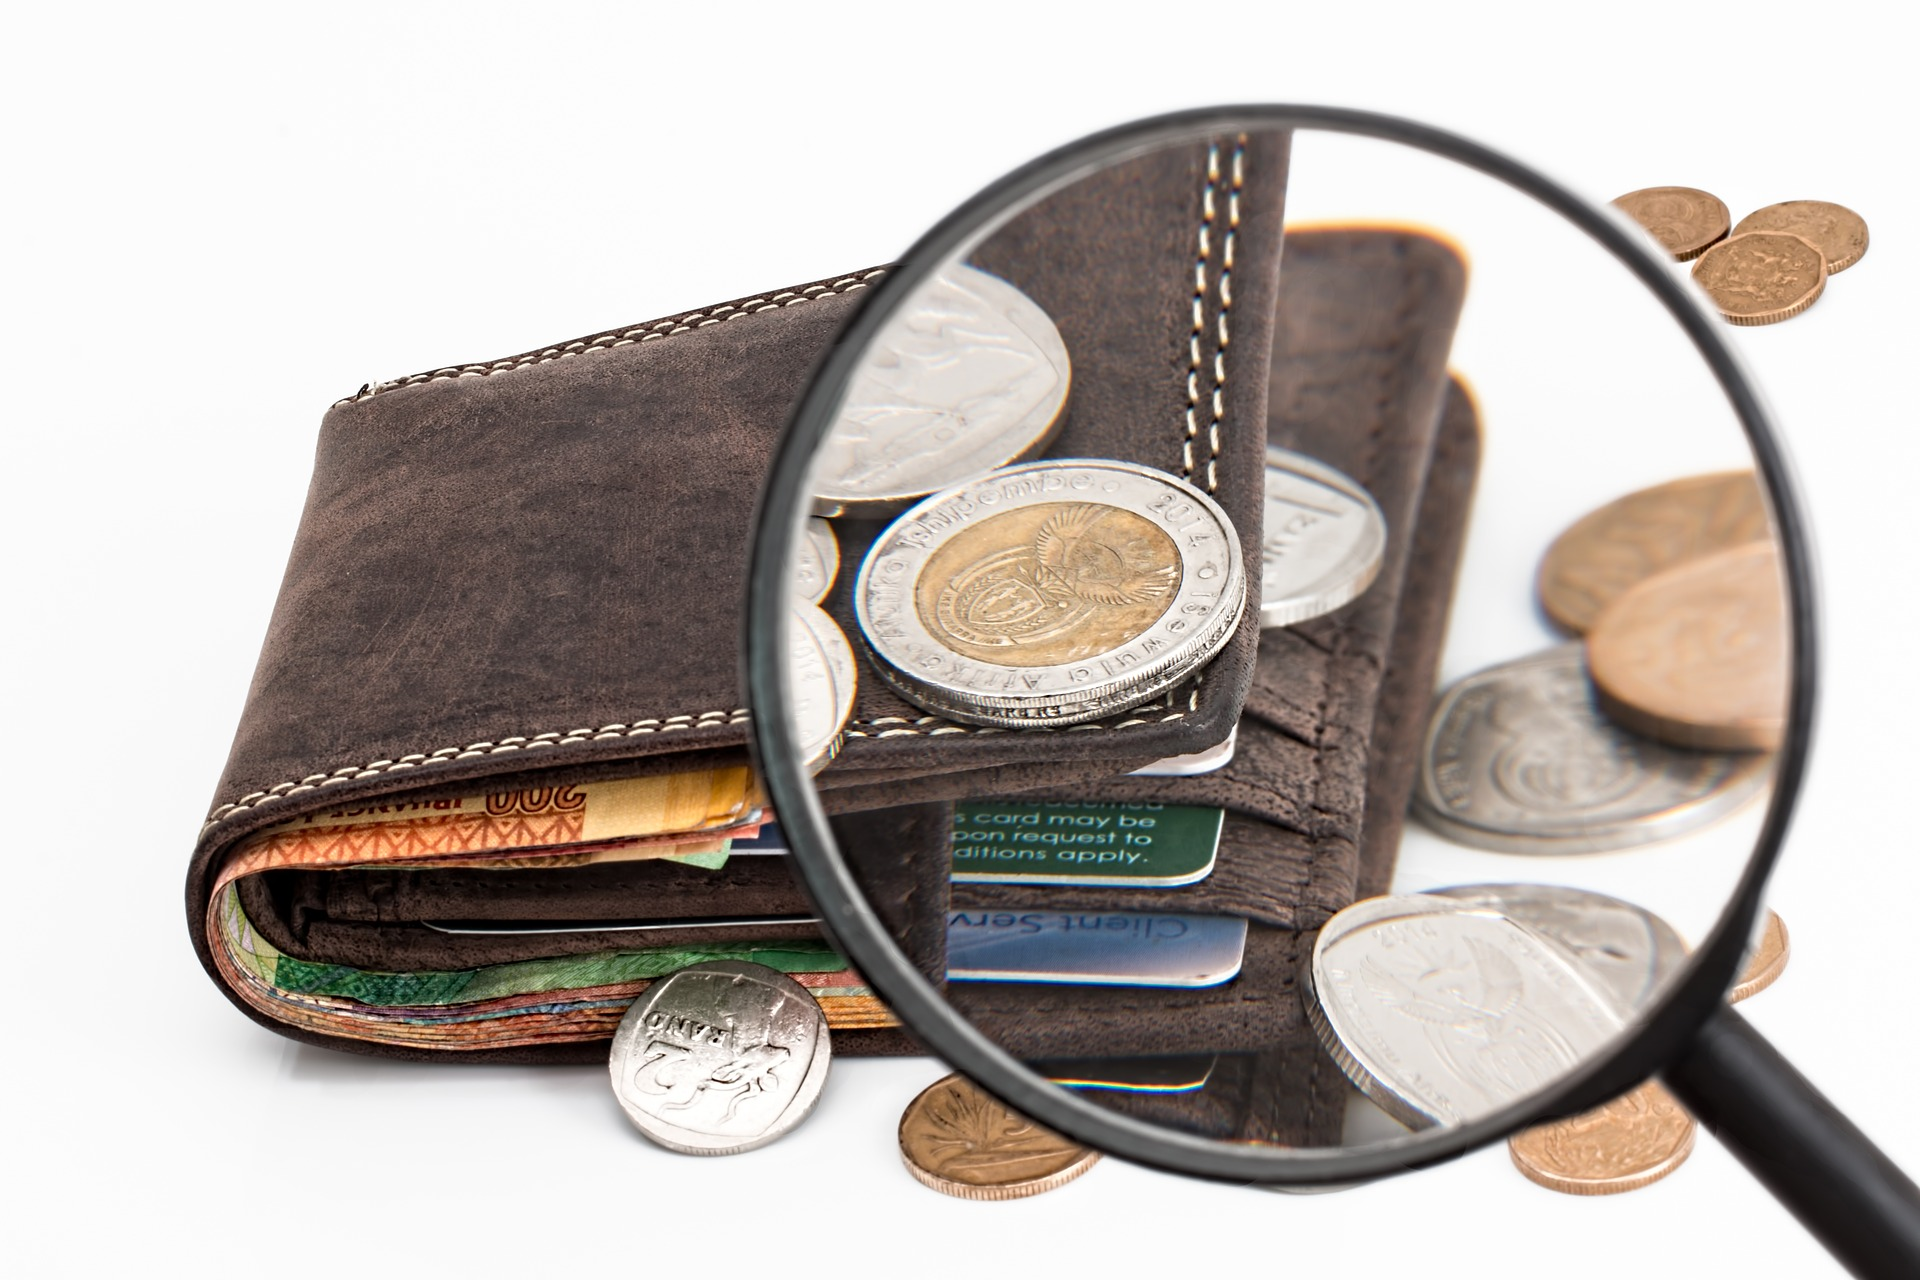
\includegraphics[width=0.3\textwidth]{Fig/profile}
%	
%\end{figure}
%
%\begin{itemize}
%  \item Very long tails of the log-returns distribution (quantiles and condition tail expectations)
%  \item High variance
%  \item High value of the alpha-stable scale parameter $S_\gamma$
%  \item Value of the alpha-stable tail index $S_\alpha$ closer to 1
%   \item Positive first order autocorrelation of log-returns
%   \item Hurst exponent higher than 0.5
%\end{itemize}
%
%
%}

\frame{
	\frametitle{Conclusion}
	
\begin{itemize}
  \item Financial perspective

	\begin{itemize}
		\item Main statistical difference between Cryptocurrencies and other asset classes: tail behavior.
		\item Moments and memory are of subliminal importance.
		\item Nonlinear classification with SVM provides proficient results for risk analysts and regulators.
		\item Cryptocurrencies are completely separated by the other types of
		assets, as proved by Maximum Variance Components Split method.
	\end{itemize}
\item Biological perspective

\begin{itemize}
  \item Speciation takes time to form distinct species, which potentially evolve further away from each other.
  \item Cryptocurrencies establish themselves as unique asset classes.
\end{itemize}
\end{itemize}	
	
}

\Section{}

\frame[plain]{% create the titleslide, layout controlled in metricsbeamer
	\titlepage}

\section{Appendix}

\frame{
\frametitle{Exchange rates} \label{sec:appendix_forex}
\vspace{-3mm}
\hyperlink{sec:data}{\beamergotobutton{Data}}
\vspace{-1mm}



\begin{enumerate}
\item EUR/USD	Euro
\item JPY/USD	Japanese Yen
\item GBP/USD	Great Britain Pound
\item CAD/USD	Canada Dollar
\item AUD/USD	Australia Dollar
\item NZD/USD	New Zealand Dollar
\item CHF/USD	Swiss Franc
\item DKK/USD	Danish Krone
\item NOK/USD	Norwegian Krone
\item SEK/USD	Swedish Krone
\item CNY/USD	Chinese Yuan Renminbi
\item HKD/USD	Hong Kong Dollar
\item INR/USD	Indian Rupee
\end{enumerate}

}




\frame{
	\frametitle{Commodities} \label{sec:appendix_Commodities}
	\vspace{-3mm}
	\hyperlink{sec:data}{\beamergotobutton{Data}}
	\vspace{-1mm}


	
		
		\begin{enumerate}
		\scriptsize
			\item 	WTI Crude oil	USCRWTIC Index
			\item 	Natural Gas	NGUSHHUB Index
			\item 	Brent oil	EUCRBRDT Index
			\item 	Unleaded Gasoline	RBOB87PM Index
			\item 	ULS Diesel	DIEINULP Index
			\item 	Live cattle	SPGSLC Index
			\item 	Lean hogs	HOGSNATL Index
			\item 	Wheat	WEATTKHR Index
			\item 	Corn	CRNUSPOT Index
			\item 	Soybeans	SOYBCH1Y Index
			\item 	Aluminum	LMAHDY Comdty
			\item 	Copper	LMCADY Comdty
			\item 	Zinc	ZSDY Comdty
			\item 	Nickel	CKEL Comdty
			\item 	Tin	JMC1DLTS Index
			\item 	Gold	XAU Curncy
			\item 	Silver	XAG Curncy
			\item 	Platinum	XPT Curncy
			\item 	Cotton	COTNMAVG Index
			\item 	Cocoa	MLCXCCSP Index
			
		\end{enumerate}

}


\frame{
\frametitle{L\'{e}vy-Stable distributions} \label{sec:appendix_stable}

\begin{itemize}
\item Fourier transform of characteristic function $\varphi_X(u)$%=\operatorname{E}\left[ \exp(itx)\right]$
\begin{equation*}
S(X\mid \alpha,\beta,\gamma,\delta)=\frac{1}{2\pi} \int \varphi_X(u) \exp(-iuX) du
\end{equation*}
\item Characteristic function representation, $0<\alpha<2, \alpha\neq 1$
\begin{equation}
\log \varphi_X(u) = iu\delta-\gamma \lvert u\rvert\ ^\alpha \left\{1+i\beta \left(u / \lvert u\rvert \right) \tan\left(\alpha\pi/2\right)\right\}
\end{equation}
\item Stability or invariance under addition
\begin{equation*}
n \log \varphi_X(u) = iu(n\delta)-(n\gamma) \lvert u\rvert\ ^\alpha \left\{1+i\beta \left(u / \lvert u\rvert \right) \tan\left(\alpha\pi/2\right)\right\}
\end{equation*}
\item Limiting distribution of $n$ i.i.d. stable r.v., $0<\alpha\leq2$ \newline GCLT (Gnedenko and Kolmogorov, 1954)
\begin{equation}
n^{-\frac{1}{\alpha}} \sum_{i=1}^n (X_i-\delta)\xrightarrow[]{\mathcal{L}} S(\alpha,\beta,\gamma,0)
\end{equation}
\end{itemize}
\hyperlink{sec:data}{\beamergotobutton{Statistical assessment}}
}

\frame{
\frametitle{Linear Discriminant Analysis} \label{sec:appendix_lda}

\begin{itemize}
  \item Let $X_i\sim N(\mu_i,\Sigma_i)$ belonging to class $\omega_i,\ \Sigma_i=\Sigma_j$
  \item Project samples $X$ onto a line $Y = w^\top X$
  \item Select the projection that maximized the separability
  \item Maximize normalized, squared distance in the means of the classes
  \begin{align}
  w^\ast=\underset{w}{\arg\max}\ \frac{\vert w^\top(\mu_i-\mu_j)\vert^2}{s_i^2+s_j^2},\\
  s_i^2=\sum_{x_i\in\omega_i}(w^\top x_i-w^\top \mu_i)^2=w^\top S_i w
  \end{align}
  \item Linear Discriminant of Fisher (1936)
  \begin{align}
  w^\ast=S_W^{-1}(\mu_i-\mu_j),\ S_W=S_i+S_j
  \end{align}
\end{itemize}

\hyperlink{sec:lda}{\beamergotobutton{LDA}}
}

\frame{
\frametitle{Support Vector Machines} \label{sec:appendix_svm}

\begin{minipage}{0.5\textwidth}
\begin{itemize}
\item Given training data set $D$ with $n$ samples and $2$ dimensions
\begin{align*}
D=\left(X_{1}, Y_{1}\right), \ldots \left(X_{n}, Y_{n}\right),\\
X_{i} \in \mathbb{R}^{2}, \quad Y_{i} \in[0,1]
\end{align*}
\item Finding a hyperplane that maximizes the margin
\begin{align*}
\min _{w, b} \frac{1}{2}\|w\|^{2}\\
\text{s.t.} \quad Y_{i}\left(w^{\top} X_{i}+b\right) \geq 1,\\ i=1, \ldots, n
\end{align*}
\end{itemize}
\end{minipage}
%\hfill
\begin{minipage}{0.45\textwidth}
\begin{figure}[!ht]
	\includegraphics[width=0.9\textwidth]{Fig/svm}
    \caption{\hyperlink{sec:svm}{\beamergotobutton{SVM}}}
\end{figure}
\end{minipage}

}


\frame{
\frametitle{Variance Component Split} \label{sec:appendix_MVCS}
\small{
\begin{itemize}

\item Consider the groups
$X_{(1)}, \ldots, X_{(i)}$ and $X_{(i+1)},\ldots, X_{(n)}$
%}
with averages, respectively,
$\bar X_{[1,i]}$    and
$\bar X_{[i+1,n]},$
$i=1,...,n-1,$
then
\begin{equation}
\label{eq:unusualANOVA}
\frac {1}{n}\sum_{i=1}^n (X_i - \bar{X})^2 =
\sum_{i=1}^{n-1} \frac {i(n-i)} {n^2}
(\bar X_{[i+1,n]}-\bar X_{[1,i]})  (X_{(i+1)}-X_{(i)}).
\end{equation}

\item The relative contribution  of the groups $X_{(1)},...,X_{(i)}$ and
$X_{(i+1)},...,X_{(n)}$   in the sample variability:
\begin{equation}
\label{eq:weights}
W_i=W_i(X_1,\ldots,X_n)
=\frac {i(n-i)} {n} \frac {(\bar X_{[i+1,n]}-\bar X_{[1,i]})
	(X_{(i+1)}-X_{(i)})} {\sum_{i=1}^n (X_i - \bar{X})^2}
\end{equation}
\item
Index ${\cal I}_n=\max \{W_i, i=1,\ldots,n-1\}$ determines two potential clusters or parts of a structure and is based  on averages and inter-point distances.
\end{itemize}
}
}

\frame{
	\frametitle{Maximum Variance Component Split} \label{sec:appendix_MVCS}
\small{	
	\begin{itemize}

\item
The Maximum Variance Component Split (MVCS) method compares known components of a structure, {\em e.g.}  cryptocurrencies herein,  with data splits for
a set of unit projection directions ${\cal D}_M$   usually determined by  $M$  positive equidistant angles of $[0,\pi];$
{\em e.g.} when $r=2$ and  $M=3$ the angles used  are $\pi/3, 2 \pi/3, \pi.$
\item When one of the  data split along  projection direction ${\bf a}$  coincides with a component of the structure we have complete separation of this component along  ${\bf a}.$

\item A set of projection directions ${\cal D}_M$ can be
\begin{equation}
(\Pi_{l=1}^rcos\theta_l, \mbox{ } sin\theta_1 \Pi_{l=2}^r cos\theta_l,...,
\mbox{ } sin\theta_{r-1}cos\theta_r, \mbox{ }
sin\theta_r),
\label{eq:discretizeddirections}
\end{equation}
where $\theta_l$ takes values in
$\{\frac{m\pi}{M}, m=1,..., M\}, l=1,...,r.$
%%%%%%%%%%%%%%%%%%%%%%%%%%%%%%%%
\end{itemize}

}
{\hyperlink{sec:MVCS}{\beamergotobutton{MVCS}}}


}
%%%%%%%%%%%%%%%%%%%%%%%%%%%%%%%%


\section{References}

%\frame{
%\frametitle{For Further Reading}
%\begin{thebibliography}{aaaaaaaaaaaaaaaaa}
%\beamertemplatearticlebibitems
%\bibitem{Kelly:1956}
%J. Kelly
%\newblock{\em A new interpretation of information rate}
%\newblock Bell System Technology Journal, 35, 1956
%\beamertemplatearticlebibitems
%\bibitem{Breiman:1961}
%L. Breiman
%\newblock{\em Optimal gambling system for favorable games}
%\newblock Proceedings of the 4th Berkeley Symposium on Mathematics, Statistics and Probability, 1, 1961
%\beamertemplatearticlebibitems
%\bibitem{Merton:1992}
%R. C. Merton
%\newblock{\em Continuous Time Finance}
%\newblock MA Blackwell Publishers Inc, 1992
%\end{thebibliography}
%}
%
%%%%%%%%%%%%%%%%%%%%%%%%%%%%%%%%%%
%
%\frame{
%\frametitle{For Further Reading}
%\begin{thebibliography}{aaaaaaaaaaaaaaaaa}
%\beamertemplatearticlebibitems
%\bibitem{mzb:1992}
%L. C. MacLean, W. T. Ziemba and G. Blazenko
%\newblock{\em Growth versus Security in Dynamic Investment Analysis}
%\newblock Management Science, 38(11), 1992
%\beamertemplatearticlebibitems
%\bibitem{Thorp:2006}
%E. O. Thorp
%\newblock{\em The Kelly criterion in Blackjack, Sports betting and the Stock Market}
%\newblock Handbook of Asset and Liability Management, 2006
%\beamertemplatearticlebibitems
%\bibitem{Nolan:2006}
%J. P. Nolan
%\newblock{\em Multivariate elliptically contoured stable distributions}
%\newblock Stable Distributions, 2006
%\end{thebibliography}
%}
%
%%%%%%%%%%%%%%%%%%%%%%%%%%%%%%%%%


\end{document}

